% Lines starting with a percent sign (%) are comments. LaTeX will
% not process those lines. Similarly, everything after a percent
% sign in a line is considered a comment. To produce a percent sign
% in the output, write \% (backslash followed by the percent sign).
% ==================================================================
% Usage instructions:
% ------------------------------------------------------------------
% The file is heavily commented so that you know what the various
% commands do. Feel free to remove any comments you don't need from
% your own copy. When redistributing the example thesis file, please
% retain all the comments for the benefit of other thesis writers!
% ==================================================================
% Compilation instructions:
% ------------------------------------------------------------------
% Use pdflatex to compile! Input images are expected as PDF files.
% Example compilation:
% ------------------------------------------------------------------
% > pdflatex thesis-example.tex
% > bibtex thesis-example
% > pdflatex thesis-example.tex
% > pdflatex thesis-example.tex
% ------------------------------------------------------------------
% You need to run pdflatex multiple times so that all the cross-references
% are fixed. pdflatex will tell you if you need to re-run it (a warning
% will be issued)
% ------------------------------------------------------------------
% Compilation has been tested to work in ukk.cs.hut.fi and kosh.hut.fi
% - if you have problems of missing .sty -files, then the local LaTeX
% environment does not have all the required packages installed.
% For example, when compiling in vipunen.hut.fi, you get an error that
% tikz.sty is missing - in this case you must either compile somewhere
% else, or you cannot use TikZ graphics in your thesis and must therefore
% remove or comment out the tikz package and all the tikz definitions.
% ------------------------------------------------------------------

% General information
% ==================================================================
% Package documentation:
%
% The comments often refer to package documentation. (Almost) all LaTeX
% packages have documentation accompanying them, so you can read the
% package documentation for further information. When a package 'xxx' is
% installed to your local LaTeX environment (the document compiles
% when you have \usepackage{xxx} and LaTeX does not complain), you can
% find the documentation somewhere in the local LaTeX texmf directory
% hierarchy. In ukk.cs.hut.fi, this is /usr/texlive/2008/texmf-dist,
% and the documentation for the titlesec package (for example) can be
% found at /usr/texlive/2008/texmf-dist/doc/latex/titlesec/titlesec.pdf.
% Most often the documentation is located as a PDF file in
% /usr/texlive/2008/texmf-dist/doc/latex/xxx, where xxx is the package name;
% however, documentation for TikZ is in
% /usr/texlive/2008/texmf-dist/doc/latex/generic/pgf/pgfmanual.pdf
% (this is because TikZ is a front-end for PGF, which is meant to be a
% generic portable graphics format for LaTeX).
% You can try to look for the package manual using the ``find'' shell
% command in Linux machines; the find databases are up-to-date at least
% in ukk.cs.hut.fi. Just type ``find xxx'', where xxx is the package
% name, and you should find a documentation file.
% Note that in some packages, the documentation is in the DVI file
% format. In this case, you can copy the DVI file to your home directory,
% and convert it to PDF with the dvipdfm command (or you can read the
% DVI file directly with a DVI viewer).
%
% If you can't find the documentation for a package, just try Googling
% for ``latex packagename''; most often you can get a direct link to the
% package manual in PDF format.
% ------------------------------------------------------------------


% Document class for the thesis is report
% ------------------------------------------------------------------
% You can change this but do so at your own risk - it may break other things.
% Note that the option pdftext is used for pdflatex; there is no
% pdflatex option.
% ------------------------------------------------------------------
\documentclass[12pt,a4paper,oneside,pdftex]{report}

% The input files (tex files) are encoded with the latin-1 encoding
% (ISO-8859-1 works). Change the latin1-option if you use UTF8
% (at some point LaTeX did not work with UTF8, but I'm not sure
% what the current situation is)
\usepackage[latin1]{inputenc}
% OT1 font encoding seems to work better than T1. Check the rendered
% PDF file to see if the fonts are encoded properly as vectors (instead
% of rendered bitmaps). You can do this by zooming very close to any letter
% - if the letter is shown pixelated, you should change this setting
% (try commenting out the entire line, for example).
\usepackage[OT1]{fontenc}
% The babel package provides hyphenating instructions for LaTeX. Give
% the languages you wish to use in your thesis as options to the babel
% package (as shown below). You can remove any language you are not
% going to use.
% Examples of valid language codes: english (or USenglish), british,
% finnish, swedish; and so on.
\usepackage[finnish,english]{babel}

% placeins allows for use of FloatBarrier, which helps with the layout of the
% results chapter
\usepackage{placeins}

% for mathstuff
\usepackage{amssymb}

% Font selection
% ------------------------------------------------------------------
% The default LaTeX font is a very good font for rendering your
% thesis. It is a very professional font, which will always be
% accepted.
% If you, however, wish to spicen up your thesis, you can try out
% these font variants by uncommenting one of the following lines
% (or by finding another font package). The fonts shown here are
% all fonts that you could use in your thesis (not too silly).
% Changing the font causes the layouts to shift a bit; you many
% need to manually adjust some layouts. Check the warning messages
% LaTeX gives you.
% ------------------------------------------------------------------
% To find another font, check out the font catalogue from
% http://www.tug.dk/FontCatalogue/mathfonts.html
% This link points to the list of fonts that support maths, but
% that's a fairly important point for master's theses.
% ------------------------------------------------------------------
% <rant>
% Remember, there is no excuse to use Comic Sans, ever, in any
% situation! (Well, maybe in speech bubbles in comics, but there
% are better options for those too)
% </rant>

% \usepackage{palatino}
% \usepackage{tgpagella}



% Optional packages
% ------------------------------------------------------------------
% Select those packages that you need for your thesis. You may delete
% or comment the rest.

% Natbib allows you to select the format of the bibliography references.
% The first example uses numbered citations:
\usepackage[square,sort&compress,numbers]{natbib}
% The second example uses author-year citations.
% If you use author-year citations, change the bibliography style (below);
% acm style does not work with author-year citations.
% Also, you should use \citet (cite in text) when you wish to refer
% to the author directly (\citet{blaablaa} said blaa blaa), and
% \citep when you wish to refer similarly than with numbered citations
% (It has been said that blaa blaa~\citep{blaablaa}).
% \usepackage[square]{natbib}

% The alltt package provides an all-teletype environment that acts
% like verbatim but you can use LaTeX commands in it. Uncomment if
% you want to use this environment.
% \usepackage{alltt}

% The eurosym package provides a euro symbol. Use with \euro{}
\usepackage{eurosym}

% Verbatim provides a standard teletype environment that renderes
% the text exactly as written in the tex file. Useful for code
% snippets (although you can also use the listings package to get
% automatic code formatting).
\usepackage{verbatim}

% The listing package provides automatic code formatting utilities
% so that you can copy-paste code examples and have them rendered
% nicely. See the package documentation for details.
% \usepackage{listings}

% The fancuvrb package provides fancier verbatim environments
% (you can, for example, put borders around the verbatim text area
% and so on). See package for details.
% \usepackage{fancyvrb}

% Supertabular provides a tabular environment that can span multiple
% pages.
%\usepackage{supertabular}
% Longtable provides a tabular environment that can span multiple
% pages. This is used in the example acronyms file.
\usepackage{longtable}

% The fancyhdr package allows you to set your the page headers
% manually, and allows you to add separator lines and so on.
% Check the package documentation.
% \usepackage{fancyhdr}

% Subfigure package allows you to use subfigures (i.e. many subfigures
% within one figure environment). These can have different labels and
% they are numbered automatically. Check the package documentation.
%\usepackage{subfigure}
\usepackage{subcaption}
% The titlesec package can be used to alter the look of the titles
% of sections, chapters, and so on. This example uses the ``medium''
% package option which sets the titles to a medium size, making them
% a bit smaller than what is the default. You can fine-tune the
% title fonts and sizes by using the package options. See the package
% documentation.
\usepackage[medium]{titlesec}

% The TikZ package allows you to create professional technical figures.
% The learning curve is quite steep, but it is definitely worth it if
% you wish to have really good-looking technical figures.
\usepackage{tikz}
% You also need to specify which TikZ libraries you use
\usetikzlibrary{positioning}
\usetikzlibrary{calc}
\usetikzlibrary{arrows}
\usetikzlibrary{decorations.pathmorphing,decorations.markings}
\usetikzlibrary{shapes}
\usetikzlibrary{patterns}



\usepackage{caption}
% The aalto-thesis package provides typesetting instructions for the
% standard master's thesis parts (abstracts, front page, and so on)
% Load this package second-to-last, just before the hyperref package.
% Options that you can use:
%   mydraft - renders the thesis in draft mode.
%             Do not use for the final version.
%   doublenumbering - [optional] number the first pages of the thesis
%                     with roman numerals (i, ii, iii, ...); and start
%                     arabic numbering (1, 2, 3, ...) only on the
%                     first page of the first chapter
%   twoinstructors  - changes the title of instructors to plural form
%   twosupervisors  - changes the title of supervisors to plural form
\usepackage[mydraft,twosupervisors]{aalto-thesis}
%\usepackage[mydraft,doublenumbering]{aalto-thesis}
%\usepackage{aalto-thesis}


% Hyperref
% ------------------------------------------------------------------
% Hyperref creates links from URLs, for references, and creates a
% TOC in the PDF file.
% This package must be the last one you include, because it has
% compatibility issues with many other packages and it fixes
% those issues when it is loaded.
\RequirePackage[pdftex]{hyperref}
% Setup hyperref so that links are clickable but do not look
% different
\hypersetup{colorlinks=false,raiselinks=false,breaklinks=true}
\hypersetup{pdfborder={0 0 0}}
\hypersetup{bookmarksnumbered=true}
% The following line suggests the PDF reader that it should show the
% first level of bookmarks opened in the hierarchical bookmark view.
\hypersetup{bookmarksopen=true,bookmarksopenlevel=1}
% Hyperref can also set up the PDF metadata fields. These are
% set a bit later on, after the thesis setup.


% Thesis setup
% ==================================================================
% Change these to fit your own thesis.
% \COMMAND always refers to the English version;
% \FCOMMAND refers to the Finnish version; and
% \SCOMMAND refers to the Swedish version.
% You may comment/remove those language variants that you do not use
% (but then you must not include the abstracts for that language)
% ------------------------------------------------------------------
% If you do not find the command for a text that is shown in the cover page or
% in the abstract texts, check the aalto-thesis.sty file and locate the text
% from there.
% All the texts are configured in language-specific blocks (lots of commands
% that look like this: \renewcommand{\ATCITY}{Espoo}.
% You can just fix the texts there. Just remember to check all the language
% variants you use (they are all there in the same place).
% ------------------------------------------------------------------
\newcommand{\TITLE}{Stream Processing on a Multicore DSP with Open Event Machine}
\newcommand{\FTITLE}{OpenEM:n Suorituskykyominaisuudet Reaaliaikaisessa Virtalaskennassa Moniydin DSP:ll�}
\newcommand{\SUBTITLE}{}
\newcommand{\FSUBTITLE}{}
\newcommand{\SSUBTITLE}{}
\newcommand{\DATE}{April 28, 2016}
\newcommand{\FDATE}{28. Maaliskuuta 2016}
\newcommand{\SDATE}{Den 28. Mars 2011}

% Supervisors and instructors
% ------------------------------------------------------------------
% If you have two supervisors, write both names here, separate them with a
% double-backslash (see below for an example)
% Also remember to add the package option ``twosupervisors'' or
% ``twoinstructors'' to the aalto-thesis package so that the titles are in
% plural.
% Example of one supervisor:
%\newcommand{\SUPERVISOR}{Professor Antti Yl�-J��ski}
%\newcommand{\FSUPERVISOR}{Professori Antti Yl�-J��ski}
%\newcommand{\SSUPERVISOR}{Professor Antti Yl�-J��ski}
% Example of twosupervisors:
\newcommand{\SUPERVISOR}{Professor Heikki Saikkonen}
\newcommand{\FSUPERVISOR}{Professori Heikki Saikkonen}
\newcommand{\SSUPERVISOR}{Professor Heikki Saikkonen}

% If you have only one instructor, just write one name here
\newcommand{\INSTRUCTOR}{Vesa Hirvisalo D.Sc. (Tech.)}
\newcommand{\FINSTRUCTOR}{TkT Vesa Hirvisalo}
\newcommand{\SINSTRUCTOR}{TkT Vesa Hirvisalo}
% If you have two instructors, separate them with \\ to create linefeeds
% \newcommand{\INSTRUCTOR}{Olli Ohjaaja M.Sc. (Tech.)\\
%  Elli Opas M.Sc. (Tech)}
%\newcommand{\FINSTRUCTOR}{Diplomi-insin��ri Olli Ohjaaja\\
%  Diplomi-insin��ri Elli Opas}
%\newcommand{\SINSTRUCTOR}{Diplomingenj�r Olli Ohjaaja\\
%  Diplomingenj�r Elli Opas}

% If you have two supervisors, it is common to write the schools
% of the supervisors in the cover page. If the following command is defined,
% then the supervisor names shown here are printed in the cover page. Otherwise,
% the supervisor names defined above are used.
\newcommand{\COVERSUPERVISOR}{Professor Heikki Saikkonen}

% The same option is for the instructors, if you have multiple instructors.
% \newcommand{\COVERINSTRUCTOR}{Olli Ohjaaja M.Sc. (Tech.), Aalto University\\
%  Elli Opas M.Sc. (Tech), Aalto SCI}


% Other stuff
% ------------------------------------------------------------------
\newcommand{\PROFESSORSHIP}{}
\newcommand{\FPROFESSORSHIP}{}
\newcommand{\SPROFESSORSHIP}{}
% Professorship code is the same in all languages
\newcommand{\PROFCODE}{T-106}
\newcommand{\KEYWORDS}{stream processing, digital signal processor, parallelism, hardware accelerated scheduling}
\newcommand{\FKEYWORDS}{}
\newcommand{\SKEYWORDS}{}
\newcommand{\LANGUAGE}{English}
\newcommand{\FLANGUAGE}{Englanti}
\newcommand{\SLANGUAGE}{Engelska}

% Author is the same for all languages
\newcommand{\AUTHOR}{Risto Vuorio}


% Currently the English versions are used for the PDF file metadata
% Set the PDF title
\hypersetup{pdftitle={\TITLE\ \SUBTITLE}}
% Set the PDF author
\hypersetup{pdfauthor={\AUTHOR}}
% Set the PDF keywords
\hypersetup{pdfkeywords={\KEYWORDS}}
% Set the PDF subject
\hypersetup{pdfsubject={Master's Thesis}}


% Layout settings
% ------------------------------------------------------------------

% When you write in English, you should use the standard LaTeX
% paragraph formatting: paragraphs are indented, and there is no
% space between paragraphs.
% When writing in Finnish, we often use no indentation in the
% beginning of the paragraph, and there is some space between the
% paragraphs.

% If you write your thesis Finnish, uncomment these lines; if
% you write in English, leave these lines commented!
% \setlength{\parindent}{0pt}
% \setlength{\parskip}{1ex}

% Use this to control how much space there is between each line of text.
% 1 is normal (no extra space), 1.3 is about one-half more space, and
% 1.6 is about double line spacing.
% \linespread{1} % This is the default
% \linespread{1.3}

% Bibliography style
% acm style gives you a basic reference style. It works only with numbered
% references.
% \bibliographystyle{acm}
% Plainnat is a plain style that works with both numbered and name citations.
\bibliographystyle{plainnat}


% Extra hyphenation settings
% ------------------------------------------------------------------
% You can list here all the files that are not hyphenated correctly.
% You can provide many \hyphenation commands and/or separate each word
% with a space inside a single command. Put hyphens in the places where
% a word can be hyphenated.
% Note that (by default) LaTeX will not hyphenate words that already
% have a hyphen in them (for example, if you write ``structure-modification
% operation'', the word structure-modification will never be hyphenated).
% You need a special package to hyphenate those words.
\hyphenation{di-gi-taa-li-sta yksi-suun-tai-sta}



% The preamble ends here, and the document begins.
% Place all formatting commands and such before this line.
% ------------------------------------------------------------------
\begin{document}
% This command adds a PDF bookmark to the cover page. You may leave
% it out if you don't like it...
\pdfbookmark[0]{Cover page}{bookmark.0.cover}
% This command is defined in aalto-thesis.sty. It controls the page
% numbering based on whether the doublenumbering option is specified
\startcoverpage

% Cover page
% ------------------------------------------------------------------
% Options: finnish, english, and swedish
% These control in which language the cover-page information is shown
\coverpage{english}


% Abstracts
% ------------------------------------------------------------------
% Include an abstract in the language that the thesis is written in,
% and if your native language is Finnish or Swedish, one in that language.

% Abstract in English
% ------------------------------------------------------------------
\thesisabstract{english}{
    Streaming data is responsible for a large fraction of the growth in creation and copying of data over the Internet. Stream processing is a computing paradigm that seeks to provide a useful abstraction of computing over streaming data. The stream processing and signal processing models are similar on a high level.

    Digital Signal Processors are computing units optimized for low energy consumption in signal processing tasks. The trend toward more cores in CPUs and GPUs has been adopted by the DSP vendors as well. Multi-core DSPs provide an interesting platform for stream processing as they combine an architecture optimized for signal processing tasks with the parallel computing power of the multiple cores.

    Scheduling parallel computing is a non-trivial task. On DSPs it is often complicated by the lack of OS as an abstraction layer for parallelism. Open Event Machine provides task-parallel computing model for Texas Instruments multi-core DSPs with a dynamic, hardware accelerated scheduler. In this thesis the performance of OpenEM in stream processing is investigated. The TI implementation of OpenEM for TMS320C6678 is used in this thesis.

    The concrete contributions of this thesis are the construction of an OpenEM based stream processing measurement system, the construction of similar, statically scheduled measurement system, the comparison of the systems and the analysis of the stream processing performance of OpenEM using the measurement systems. The analysis uses the results of three experiments conducted in this thesis.

    The results of the experiments show that OpenEM runtime can be used for implementing high performance stream processing applications. Further research is needed to compare the performance to the competing computing platforms.
}

% ------------------------------------------------------------------
\thesisabstract{finnish}{}

% Acknowledgements
% ------------------------------------------------------------------
% Select the language you use in your acknowledgements
\selectlanguage{english}

% Uncomment this line if you wish acknoledgements to appear in the
% table of contents
%\addcontentsline{toc}{chapter}{Acknowledgements}

% The star means that the chapter isn't numbered and does not
% show up in the TOC
\chapter*{Acknowledgements}
\vskip 10mm

\noindent Espoo, \DATE
\vskip 5mm
\noindent\AUTHOR

% Acronyms
% ------------------------------------------------------------------
% Use \cleardoublepage so that IF two-sided printing is used
% (which is not often for masters theses), then the pages will still
% start correctly on the right-hand side.
\cleardoublepage
% Example acronyms are placed in a separate file, acronyms.tex
\addcontentsline{toc}{chapter}{Abbreviations and Acronyms}
\chapter*{Abbreviations and Acronyms}

% The longtable environment should break the table properly to multiple pages,
% if needed

\noindent
\begin{longtable}{@{}p{0.25\textwidth}p{0.7\textwidth}@{}}
    4CIF & 4 x CIF \\
    API & Application Programming Interface \\
    CCS & Code Composer Studio \\
    CIF & Common Intermediate Format \\
    CPU & Central Processing Unit \\
    DDF & Dynamic Dataflow \\
    DDR & Double Data Rate \\
    DMA & Direct Memory Access \\
    DPDK & Dataplane Development Kit \\
    DSP & Digital Signal Processor \\
    EMIF & External Memory Interface \\
    EO & Execution Object \\
    FLOPS & Floating-point Operations Per Second \\
    FPGA & Field-Programmable Gate Array \\
    GPU & Graphics Processing Unit \\
    IDE & Integrated Development Environment \\
    L1 & Level 1 cache \\
    L2 & Level 2 cache \\
    MCSDK & Multicore Software Development Kit \\
    MPEG & Moving Picture Experts Group \\
    MSM & Multicore Shared Memory \\
    MSMC & Multicore Shared Memory Controller \\
    MoC & Model of Computation \\
    NSN & Nokia Solutions and Networks \\
    NTSC & National Television System Committee \\
    OpenEM & Open Event Machine \\
    PCI & Peripheral Component Interconnect \\
    PDSP & Packed Data Structure Processor \\
    PKTDMA & Packet Direct Memory Access \\
    PiSDF & Parameterized and Interfaced Synchronous Dataflow \\
    QCIF & Quarter CIF \\
    RGB & Red Green Blue \\
    S-LAM & System-Level Architecture Model \\
    SDF & Synchronous Dataflow \\
    SoC & System on a Chip \\
    TI & Texas Instruments \\
    UI & User Interface \\
    YCbCr & YCbCr color space \\
    YUV & YUV color space \\
\end{longtable}


% Table of contents
% ------------------------------------------------------------------
\cleardoublepage
% This command adds a PDF bookmark that links to the contents.
% You can use \addcontentsline{} as well, but that also adds contents
% entry to the table of contents, which is kind of redundant.
% The text ``Contents'' is shown in the PDF bookmark.
\pdfbookmark[0]{Contents}{bookmark.0.contents}
\tableofcontents

% List of tables
% ------------------------------------------------------------------
% You only need a list of tables for your thesis if you have very
% many tables. If you do, uncomment the following two lines.
% \cleardoublepage
% \listoftables

% Table of figures
% ------------------------------------------------------------------
% You only need a list of figures for your thesis if you have very
% many figures. If you do, uncomment the following two lines.
% \cleardoublepage
% \listoffigures

% The following label is used for counting the prelude pages
\label{pages-prelude}
\cleardoublepage

%%%%%%%%%%%%%%%%% The main content starts here %%%%%%%%%%%%%%%%%%%%%
% ------------------------------------------------------------------
% This command is defined in aalto-thesis.sty. It controls the page
% numbering based on whether the doublenumbering option is specified
\startfirstchapter

% Add headings to pages (the chapter title is shown)
\pagestyle{headings}

% The contents of the thesis are separated to their own files.
% Edit the content in these files, rename them as necessary.
% ------------------------------------------------------------------
\chapter{Introduction}
\label{chapter:intro}

\section{Problem statement}

\section{Structure of the Thesis}
\label{section:structure} 


\chapter{Data Streams}
\label{chapter:streams}
The amount of digital data that is being created and copied is increasing at a massive pace. EMC Digital Universe study \cite{turner2014digital} estimates that the data we create and copy annually was 4.4 zettabytes in 2013 and is going to reach 44 zettabytes by 2020. A large portion of this data growth is due to increased volume of entertainment in the form of audio and video being streamed through internet. New data sources such as embedded sensors are contributing to the explosive data growth as well. Most of the data being created or copied is transient and thus does not require long term storage.~\cite{turner2014digital}

Distributed data processing systems such as Hadoop~\cite{white2012hadoop} were developed for batch processing of Big Data. The batch processing systems are capable of processing massive amounts of data but the processing has high latency. As most of the growth in data creation and copying is coming from data that is not stored, batch processing is not the optimal processing method for data.

Consider live streaming of video as an example of modern application with specific data processing needs. The data is being generated by a camera filming a live scene and the users expect to access the video stream over the internet with low latency. Many distinct processing steps are required in order to get the video frames from the camera to the viewer, all of which need to be performed in few milliseconds on the frames flowing past the processing unit. In addition to video streams many other kinds of data streams which have similar processing needs are produced at an accelerating pace. Certain technologies developed for processing the streaming data are grouped under the term stream processing.

An introduction to stream processing and selected stream processing techniques are given in this chapter. A stream processing overview is given in \ref{sec:stream-processing}. Selected streaming applications and their common features are described in \ref{subsec:streaming-applications}. Platforms used for stream processing are introduced in~\ref{subsec:stream-processing-platforms}. Video streams are discussed as an example of a common type of streaming data in \ref{subsec:video-streams}. Dataflow Models of Computation are discussed in \ref{subsec:dataflow-moc} as an example of solution for stream processing. Variations of dataflow MoC are examined, synchronous dataflow in \ref{subsec:synchronous-dataflow} and dynamic dataflow in \ref{subsec:dynamic-dataflow}.

\section{Stream Processing}
\label{sec:stream-processing}
Stream processing is a method of computing over streaming data. Stream processing is often used to refer to the programming paradigm that follows the stream processing method but stream processing is not limited to the creation of software. Stream processing term has been used in the literature to describe different kinds of methods that deal with streaming data. In the context of this thesis the broad definition of stream processing as a method of processing any kind of streaming data is used. 

Stream processing paradigm defines modules that compute in parallel and communicate data via channels. The modules can be divided into three classes according to their placement and purpose in the process. The classes are sources, filters and sinks. Sources act as the input points that pass data into the process. Filters perform atomic computations on the streams. Sinks are used to pass the data out from the process.~\cite{stephens1997survey}

In stream processing the channels of communication between the modules are called streams. Streams can be described as infinite lists of elements taken from a dataset $A$. Mathematical formalization of a stream is a function $f:T \rightarrow A$ where $T = \mathbb{N}$ represents discrete time.~\cite{stephens1997survey} For example the input stream of a signal processing application can be the sample based input sequence which has been generated by sampling a sensor at fixed time intervals.

Systems built following the stream processing method can be categorized under stream processing systems. The stream processing survey by Stephens \cite{stephens1997survey} categorizes \textit{dataflow systems}, \textit{reactive systems}, \textit{synchronous concurrent algorithms}, \textit{signal processing systems}, and some \textit{real-time systems} as stream processing systems. 

\subsection{Applications of Stream Processing}
\label{subsec:streaming-applications}
The authors of the StreamIt language~\cite{thies2002streamit} have defined \textit{streaming applications} as a class of programs, that commonly have many of the features defined in the following listing.

\begin{itemize}
    \item \textit{Large streams of data.} A streaming application operates on large, virtually infinite streams of data.
    \item \textit{Independent stream filters.} The filters of a streaming application are generally self-contained. They perform atomic operations on the stream.
    \item \textit{A stable computation pattern.} A streaming application has a steady state of operation during which the graph formed by the filters remains mostly constant.
    \item \textit{Occasional modification of the stream structure.} A streaming application can occasionally modify the processing graph as a reaction to changed input or some other condition.
    \item \textit{Occasional out-of-stream communication.} The high volume communication between the filters is handled through the streams but the filters may communicate small amount of control data outside the stream.
    \item \textit{High performance expectations.} There often are real-time and power consumption constraints on streaming applications. For example a streaming video decoder has to decode the stream at rate of input in order to avoid unbounded buffer growth or frame dropping.
\end{itemize}

Applications that handle streams of audio and video often have the above features and can be implemented following the stream processing paradigm. The multimedia domain is therefore full of examples of stream processing applications. Video conferencing is a commonly used example of a streaming application. Streaming video decoding is used in online video streaming services. Audio streams are encoded and decoded in mobile devices for calls but also in streaming of music.

In addition to multimedia, streaming data is often encountered in other kinds of internet services as well. For example efficient computation of analytics from search engine data can be implemented using stream processing. The total dataset may be quite large and a batch computing system computing over the complete data would provide results with high latency. A stream processing system however would be able to compute the analytics from the data as the data is being produced and update the analytics separately for each piece of data received. Google has developed the MillWheel framework for implementation of such analytics~\cite{tyler2013millwheel}.

\subsection{Stream Processing Platforms}
\label{subsec:stream-processing-platforms}
A diverse variety of stream processing applications may run on different platforms ranging from phones to servers. Software stream processing systems may execute on arbitrary hardware, but to achieve good performance some platforms are preferred over the others. Stream processing is well suited for designing applications for GPUs and DSPs. The modules of stream processing can often be executed in parallel allowing for efficient use of the multiple cores of GPUs, for example~\cite{goddeke2011fast} makes use of GPUs for solving simulations involving partial differential equations using GPUs.

Digital signal processing applications are often designed in stream processing pattern and this is also reflected in the hardware making DSPs potentially powerful stream processing units~\cite{lee2015introduction}. Multi-core DSPs such as the Texas instruments TMS320C6678 used in this thesis have the potential for efficient stream processing, because they combine the DSP architecture suitable for stream processing with the parallel processing capabilities of the multiple cores.

In the software world the expression power of stream processing paradigm has been recognized and many tools have been created for the development of stream processing applications. Examples of stream processing frameworks for distributed computing are Google MillWheel~\cite{tyler2013millwheel}, Apache Storm~\cite{apache2016storm} and Apache Spark Streaming~\cite{apache2016spark}. StreamIT introduced in~\cite{thies2002streamit} is a programming language specifically for stream processing. Streaming Concurrent Collections~\cite{sbirlea2011scnc} is a stream processing system based on the Concurrent Collections~\cite{budimlic2010concurrent} programming model.

In addition to the software stream processing systems studied in this thesis, the increasing volume of streaming data has motivated research for hardware stream processors. Processor architectures that implement stream processing concepts in the hardware have been researched in Imagine \cite{kapasi2002imagine} and Merrimac~\cite{dally2003merrimac} projects at Stanford University.

\subsection{Video Streams}
\label{subsec:video-streams}
Video streams are a prime example of streaming data. In the case of streaming service such as Netflix, the video data is downloaded from the service providers server and decompressed on the device of the consumer. In most use cases the video streams are decompressed as they are downloaded and the complete video file is not necessarily stored on the device. Thus stream processing is well suited for video stream decompression. The video streams are often accompanied by audio streams, which are processed similarly.~\cite{richardson2002video}

The video conference use case is similar to the streaming video services but involves extra complexity with the compression of the raw data coming from the video camera and especially the requirement of low latency in the compression, decompression and communications.

A large fraction of the growth of data creation can be attributed to video streams. More than billion hours of TV and movies are streamed through the video streaming service Netflix \cite{turner2014digital}. Video streams are used for real-time communication through services such as Skype and Periscope. In addition to the number of users accessing the streams growing the bit rate of the streams is growing as well. The efficiency of video stream processing is thus a top priority in the industry.

\section{Dataflow}
\label{sec:dataflow-models}
Stream processing defines the high level structure of how streaming data is to be processed but it does not define the stream processing methods in detail. On high level the structure defined by dataflow models of computation corresponds well to stream processing. Looking at dataflow as the model of computation for stream processing is thus potentially useful. In this section the dataflow models of computation are examined.

\subsection{Dataflow Models of Computation}
\label{subsec:dataflow-moc}
Dataflow models of computation can be used to describe stream processing applications. In programs following a dataflow MoC, the computation can be described by a directed graph. The nodes of the graph are the computation kernels. The data being processed by the application is split into tokens which flow from node to node along the directed arcs. The only means of communication between the nodes are the data tokens. This means the dependencies of a node are necessarily satisfied as soon as it has received its input tokens, and it may begin executing. The execution of the nodes is thus asynchronous.~\cite{lee2015introduction}

To allow asynchronous execution of the nodes the tokens are buffered between the nodes. A common requirement of MoCs used in signal or stream processing is the capability of executing for an undetermined amount of time. Execution without determinate end is called unbounded execution and it means that the length of the input may be arbitrarily large. The token buffering combined with the required capability for unbounded execution leads to a possibility of unbounded buffer growth. Unbounded buffer growth is one of the main problems the different dataflow MoCs try to solve. The other main problem is the schedulability of the dataflow graph. If the graph has cycles, the model may deadlock when one of the nodes has an insufficient number of input tokens and cannot proceed execution. This keeps the nodes that come after it from receiving input and thus deadlocking the graph.~\cite{lee2015introduction}

The scheduling of dataflow graphs means determining when and where the nodes execute. The execution of the nodes is dependent on the availability of data, which places restrictions on the possible schedules. The availability of data means that the node must have the specified number of tokens in each of its input queues in order to execute. Depending on the system there may be one or more cores available for execution of the nodes. For parallel systems the nodes may execute in parallel if a parallel schedule can be found that respects the data availability constraints of the graph. Communication between cores may introduce overhead that the scheduler must be aware of in order to generate efficient schedules.~\cite{lee1987synchronous}

\subsection{Synchronous Dataflow}
\label{subsec:synchronous-dataflow}
\FloatBarrier
One approach to solving the schedulability and the unbounded buffer growth of the dataflow MoC is fixing the production and consumption rates of the actors. These limitations are implemented in the family of dataflow models introduced by Lee and Messerschmit called synchronous dataflow (SDF)~\cite{lee1987synchronous}. An SDF model imposes strict limits on the kinds of dataflow graphs allowed. The dataflow graphs in SDF models are fixed at compile time. No new actors may be added in run time to SDF graphs because all arcs of the model are fixed. The flow of tokens along the arcs is fixed as well, due to the fixed production and consumption rates of the model. Creating graphs adhering to these limitations, the graphs are fully schedulable at compile time and they execute the same way on each iteration. This means that the boundedness of the buffers is guaranteed and the deadlocking problems are avoided. Implementing such limitations reduces the expression power of SDF models compared to more lax dataflow models such as the dynamic dataflow discussed in~\ref{subsec:dynamic-dataflow}.~\cite{lee2015introduction}

\begin{figure}[h!]
    \begin{center}
        \includegraphics[width=0.40\textwidth]{images/sdf_graph.pdf}
        \caption{A SDF Graph from \cite{ade1997data}. The production rate of each connection is marked at the beginning of the arcs connecting the nodes and the consumption rates are marked respectively at the end of each arc.}
        \label{fig:sdf_graph}
    \end{center}
\end{figure}

The SDF MoC was specifically designed for digital signal processing applications. In domains such as digital signal processing the typical tasks can be presented as sequence of operations performed on an infinite stream of data, which makes them computable with SDF models. The SDF models provide good performance and guarantee deadlock-free execution and are thus often a practical choice for DSP applications.~\cite{lee2015introduction}

\begin{table}
    \begin{center}
        \begin{tabular}{ c c }
            Arc & Buffer Size \\ \hline
            ab  & 5 \\ \hline
            ac  & 10 \\ \hline
            bd  & 2 \\ \hline
            cd  & 10 \\ \hline
            ce  & 12 \\ \hline
            cf  & 30 \\ \hline
            df  & 6 \\ \hline
            ef  & 8 \\ \hline
        \end{tabular}
        \caption{The minimum required buffer sizes for the arcs in the SDF graph \ref{fig:sdf_graph}. The buffer sizes are presented as the maximum number of tokens the buffer fits. The buffers store the tokens that are waiting to be processed by the node in the receiving end of each arc.}
        \label{tab:sdf_buffers}
    \end{center}
\end{table}

Figure~\ref{fig:sdf_graph} presents an example acyclic SDF graph from~\cite{ade1997data}. The graph nodes are marked with letters from a to f and the production and consumption rates are marked at the ends of the arcs. The graph can be scheduled in many different ways, which yield different performance characteristics in terms of memory requirements of the buffers, latency and throughput. The task of scheduling and allocating buffers for SDF graphs is non-trivial. Larger buffer sizes allow for more scheduling freedom but on certain targets such as FPGAs there are severe limitations on the number of registers available for the buffer allocation. The minimum required buffer sizes that guarantee the existence of deadlock-free schedule are represented in table~\ref{tab:sdf_buffers}. The buffer sizes were found using the algorithm from~\cite{ade1997data}. For some schedules that would yield improvements in throughput or latency, larger buffer sizes may be required.

Examples of practical implementations of the SDF MoC include the parameterized and interfaced synchronous dataflow (PiSDF) used by PREESM described in~\ref{subsec:preesm-internal}, the Ptolemy project \cite{ekerjanneck2003ptolemy} and the LUSTRE programming language~\cite{halbwachs1991synchronous}.

\FloatBarrier
\subsection{Dynamic Dataflow}
\label{subsec:dynamic-dataflow}
Synchronous dataflow may be a good fit for simple signal processing tasks such as signal filtering, but it is too restricted for efficiently describing more complicated algorithms. Multiple models of computation that share the basic structure of dataflow models have been developed for more advanced needs. Dataflow models of computation that relax the constraints on token production and consumption are grouped under the name dynamic dataflow. Dynamic dataflow does not refer to a single model of computation but a group of models that differ in terms of expression power and analysability.~\cite{bhattacharyya2013handbook}

The dynamic dataflow models of computation do not constrain the number of tokens produced or consumed by an actor in a single firing. The actors may produce and consume different numbers of tokens on different firings. Relaxation of these constraints improves the expression power of the model but makes the analysis more difficult. In the class of dataflow models where these constraints have been lifted the boundedness of the buffers and the deadlocks in cyclic graphs are undecidable~\cite{buck1993scheduling}. Many dynamic dataflow models introduce other kinds of restrictions to replace the constraints on production of tokens. By limiting the types of the actors and available graph patterns dynamic dataflow models with decidable buffer growth and schedules are possible \cite{bhattacharyya2013handbook, gao1992well}. Choosing which dynamic dataflow model to use is about finding the right tradeoff between analysability and expression power for the specific application.

Dynamic dataflow is suitable for processing streams of complex data, such as compressed audio or video. A common example use case for DDF in the literature is the decoder of an MPEG video stream~\cite{bhattacharyya2013handbook}. CAL actor language supports DDF MoC and it is used by the reconfigurable video coding working group to describe the MPEG encoder and decoder~\cite{bhattacharyya2011overview}. A more recent example of using DDF in practice is the TensorFlow machine learning framework developed by Google~\cite{tensorflow2015-whitepaper}.

\chapter{Open Event Machine}
\label{chapter:openem}
This thesis investigates the performance of Open Event Machine (OpenEM) for stream processing. OpenEM is a programming framework for creating task parallel multi-core applications. Nokia Solutions and Networks (NSN) originally developed it for the networking dataplane~\cite{openemintro}.

In this chapter the OpenEM framework is introduced. To get a good view of the background of the framework, parallel computing is discussed in~\ref{sec:parallel-computing}. The section about parallel computing contains descriptions of task parallelism, which is the form of parallelism implemented by OpenEM and event-driven programming, which is the model of concurrency used in OpenEM. After the context has been introduced two views to the OpenEM framework are provided. First, the OpenEM framework as specified by Nokia is described in \ref{sec:emframework}. Second, the Texas Instruments implementation of the OpenEM framework for TMS320C6678 is explained in~\ref{sec:tiopenem}.

\section{Parallel Computing}
\label{sec:parallel-computing}
The single-thread performance of computer hardware grew rapidly, even exponentially, for many decades. This growth was reflected in software development where many software developers mainly focused on developing single-threaded programs. The main driver of single threaded performance was the increasing clock-speed of the CPUs. These increases in clock-speed slowed down around 2005 and hardware manufacturers turned more of their focus toward multi-cores. While parallel computing has been researched and practiced for decades, its importance has grown greatly after the proliferation of multi-core processors.~\cite{sutter2005free}

The OpenEM model of parallelism is described in detail in this section. In subsection~\ref{subsec:task-parallelism} a closer look is taken into task parallelism, which is the form of parallelism implemented by the OpenEM framework. In subsection~\ref{subsec:event-driven-programming} event-driven programming, which is a model of concurrency used in OpenEM, is examined.

\subsection{Task Parallelism}
\label{subsec:task-parallelism}
Task parallelism is a form of parallelism, in which units of work are distributed among multiple cores. The units of work in task parallelism are called tasks. The tasks consist of code and data in contrast to data parallelism where the same work is performed on multiple pieces of data.~\cite{hennessy2011computer} Task parallelism can be flexibly used to construct parallel programs, as the different tasks can consist of work unrelated to each other. This makes task parallelism useful with handling irregular parallelism~\cite{ayguade2009design}. The coupling results in overhead compared to data parallel models, and thus the grain size of computation needs to be sufficiently large for efficient task parallelism~\cite{subhlok1993exploiting}.

Programming frameworks that provide task parallelism generally provide ways to declare dependencies between the tasks. By implementing task dependencies the programmer may avoid having to manually synchronize the threads of execution. The task scheduler is not aware of the contents of the tasks and thus accessing shared memory inside the tasks that do not have the appropriate dependencies leads to data races and acquiring locks may lead to deadlocks. For these reasons defining dependencies between tasks is the natural way of synchronization in task parallel programs. Introduction of dependencies between the tasks limits the possible orders of execution. With enough dependencies the only possible schedule may be executing the tasks sequentially. Therefore, the dependencies between the tasks have large impact on the performance of task parallel programs and therefore unnecessary dependencies should be avoided.~\cite{hennessy2011computer}

Examples of task parallel libraries and programming languages include the Grand Central Dispatch by Apple~\cite{sakamoto2012grand}, OpenMP implements tasks from version 3.0 onwards~\cite{ayguade2009design}, Intel Thread Building Blocks~\cite{pheatt2008intel}, Cilk~\cite{blumofe1996cilk}, .Net Parallel Extensions~\cite{leijen2009design} and Habanero-Java~\cite{barik2009habanero}.

\subsection{Event-driven Programming}
\label{subsec:event-driven-programming}
Along with parallelism, concurrency is becoming more and more common in modern computing. Reasons for increasing concurrency in programs are handling asynchronous IO and responding to external events such as user interactions.

In general, IO operations consist of three phases. In the first phase, CPU sets up the operation by deciding what is read or written and where. The target hardware could be for example the hard drive of the device. In the second phase, the CPU waits for the operation to complete and has nothing to do with regards to the particular operation. In the third phase, the CPU is notified of the availability of results and begins processing them. Only phases one and three require active processing from the CPU.~\cite{friesen2015asynchronous} IO operations often take long compared to computation on the CPUs. In IO heavy applications multiple IO operations can be started concurrently and their results be processed in the order of completion. Such concurrent waiting increases the CPU utilization, as the CPUs are not spending time busy waiting for IO but instead processing the results of completed IO operations.~\cite{dabek2002event}

A common way of enabling concurrency in programs is to split the execution of the program across multiple software threads. Using threads for concurrent programming is convenient because they allow interleaving IO and computation while preserving the appearance of a serial program. A separate thread could be spawned for each IO operation so that a non-blocked thread can execute while the IO thread is waiting. The use of threads has disadvantages; for example, they introduce concurrency even to sections of programs where it is not needed. Programming with threads requires explicit synchronization of the threads, which in practice yields data races and deadlocks. Spawning software threads consumes processing cycles and memory making full software threads often heavier than necessary for the task in hand.~\cite{dabek2002event, lee2006problem}

Concurrent processing of IO and UI generated events does not necessitate the spawning of a thread for each operation. Another way of handling concurrent events is by registering an event handler with a central system that keeps track of completed operations. Such central system is commonly called the event loop. The event loop checks the completion of operations and calls the registered event handlers when the results are available. For example the Node.js~\cite{tilkov2010node} and Apple's Grand Central Dispatch~\cite{sakamoto2012grand} frameworks make use of such model of concurrency. The event-driven concurrent programming model leaves the mapping of event loops and details of how events are dispatched to its implementations. One or more threads can execute event loops and the events can even be dispatched from one thread to another depending on the implementation.

Dabek et al. argue for the use of events instead of threads to provide concurrency in IO heavy server environments. The benefits of events are that they provide comparable concurrency as threads in concurrent IO programs but are easier to program and tend to yield more stable performance under heavy loads.~\cite{dabek2002event} This along with the other advantages of events in concurrent programming have generated enough interest that many event-driven processing concepts have been developed. Here are some examples. Event-driven runtime with its own programming language called Eve has been developed by Fonseca et al.~\cite{fonseca2014eve}. Node.js~\cite{tilkov2010node} implements event-driven processing. Majority of the UI libraries such as QT~\cite{blanchette2006cpp} are implemented in an event-driven pattern.

\section{OpenEM Framework}
\label{sec:emframework}
The OpenEM framework provides a programming model for scalable and dynamically load balanced applications. OpenEM model of parallelism is task parallelism with the distinct feature that it separates the task code and data to different entities. The OpenEM tasks are scheduled using a dynamic scheduler that queues the events for one or more cores running the event loop. The Texas Instruments implementation of OpenEM uses hardware accelerators for the scheduling and inter-core communication.

The key components of the OpenEM programming model are events, execution objects, queues and the scheduler. OpenEM operates with so-called run-to-completion principle. The run-to-completion principle means that once an event starts executing it will not be interrupted. New events cannot be scheduled until a core has completed its current task even if the events in execution had lower priorities than the events forced to wait. This implies limitations within which well performing applications must be designed. The program has to be divided to small events, so that the scheduler may efficiently distribute the computation and adhere to scheduling rules and priorities. Another limitation implied by the run-to-completion principle is that the application needs to be implemented lock-free for good performance.~\cite{openempage}

The OpenEM framework structure and functionality are loosely defined by the source code distribution available at \cite{openempage}. Apart from the source distribution, there exists no public declaration of the structure and functionality of the framework. This lack of detail is explained by the OpenEM design principles, which are stated in the OpenEM source files at \cite{openempage}. A selection of the design principles is presented here. The following list is not in any particular order.

\begin{itemize}
    \item OpenEM has been designed to be \emph{easy to implement on different multi-core SoCs}.
    \item \emph{Easy integration with modern hardware accelerators} is stated to have been a major driver in the OpenEM concept design.
    \item \emph{All of the calls in the OpenEM API are multi-core safe} meaning no data structure gets broken if multiple cores make calls simultaneously. However the application designer needs to take the parallelism into consideration with regards to the application data structures and execution order.
    \item \emph{The API attempts to guide the application designer towards portable architecture.}
    \item \emph{The API is not defined for portability through recompilation.}
    \item \emph{OpenEM does not implement a full software platform or a middleware solution.} OpenEM implements a driver-level layer of such a solution but can be used by the application directly for best performance.
\end{itemize}

Another factor explaining the loose definitions is how NSN views the status of its own public OpenEM implementation targeted for Intel DPDK. The disclaimer in the NSN source distribution at \cite{openempage} states: ``The implementation of OpenEM for Intel CPUs in this package should NOT be considered a `reference OpenEM implementation', but rather an `example of an all-SW implementation of OpenEM for Intel CPUs'.'' This helps put the differences between the OpenEM API specification and the TI OpenEM implementation introduced in \ref{sec:tiopenem} in context.

The next sections will introduce the key concepts of OpenEM framework as described in the OpenEM source distribution at \cite{openempage}. The unit of communication in OpenEM is the Event described in \ref{subsec:event}. Events are sent to Queues (\ref{subsec:queues}). Queues are connected to Execution Objects (\ref{subsec:eos}). The scheduler (\ref{subsec:schedule}) chooses an event from a suitable queue based on scheduling rules and schedules it on a core. Finally, an abstract example of using OpenEM for network packet processing is given in \ref{subsec:example}.

\subsection{Events}
\label{subsec:event}
In the core of the OpenEM framework design is the event. Events are simply pointers to application specific data structures that define the communication between the different parts of the application. The application creates events and tells the framework where the event is to be passed by enqueueing it in a queue. The scheduler observes the state of the queues in the application and schedules execution objects for execution when there are events available in the queues connected to the execution objects.~\cite{openemintro}

OpenEM does not specify the event content to allow for the OpenEM implementations for different hardware platforms to organize the communication in the most efficient way available. The communication may be handled for example by hardware accelerated inter-core communication units or through simple shared memory. Usually events carry pointers to messages but they may also represent tokens for the scheduler with no data payload.~\cite{openemintro} Event memory is managed by OpenEM, meaning the application allocates events from OpenEM and freeing the events returns the control of the memory to the framework \cite{openemintro}.

OpenEM includes a fork-join helper called \textbf{event groups}. Event groups track the completion of the events sent to the group and send a notification event once a predetermined number of events have completed. The events belonging to an event group execute independently of each other and depending on other scheduling rules may execute on different cores. \cite{openemintro}

\subsection{Execution Objects}
\label{subsec:eos}
The execution objects contain the application logic. The application is built from execution objects connected by queues. Multiple queues can be connected to an execution object and an execution object may execute on multiple cores if the queueing rules allow. There are multiple possible queue configurations, which allow the execution objects to be executed on multiple cores, the main method is through the use of parallel queues.~\cite{openemintro}

The application logic for each execution object is implemented in three functions, namely start, receive, and stop. Execution object construction and destruction are handled in the application defined start and stop functions. An execution object can be scheduled on a core if there are events in the queues attached to it. When an execution object is scheduled for execution, one of the events in the queues attached to it is dequeued and passed to the receive function. Once the execution object has been scheduled on a core, it will run until the receive function returns.~\cite{openemintro}

OpenEM passes a pointer to a user defined context when calling the receive function. The application designer has complete freedom over the execution object context contents as the OpenEM runtime only passes a user defined pointer.~\cite{openemintro} If the execution object is connected to a parallel queue or multiple atomic queues, the execution object may execute on multiple cores simultaneously and thus the execution object context is shared between the cores. This limits the use of execution object context for content that has to be updated by the execution object, as the use of locks may cause the application to deadlock and is thus discouraged.

\subsection{Queues}
\label{subsec:queues}
The communication between the execution objects of an OpenEM application is handled using events. The execution objects send events to first in first out queues, which are attached to other execution objects. The scheduler selects which queue to pick events from for execution based on queue properties. The properties of the queues that affect scheduling are queue priorities, queue types and queue groups.~\cite{openemintro} The queues define what can be executed in parallel and in which order the different execution objects are executed for a given event, therefore constituting the high-level schedule of the application.

A queue is always attached to a single execution object and it cannot be attached to anything else. The behavior of queues left unattached to execution objects is not defined in the OpenEM framework. An exception to this is the unscheduled queue, which cannot be attached to execution objects, or anything else. An execution object may have one or more queues attached to it.~\cite{openemintro}

There are four types of queues: atomic, parallel, parallel ordered and unscheduled \cite{openemintro}. Only one event from an \textbf{atomic queue} may be scheduled at a time. As the use of locks is discouraged, atomic queues are the preferred way to control the access to shared memory locations. Events from \textbf{parallel queues} can be scheduled on any core at any time according to other scheduling rules explained in section \ref{subsec:schedule}. Events received from a \textbf{parallel ordered queue} are scheduled like events from parallel queues but OpenEM will restore the event ordering before events are forwarded to other queues even if the processing of the events ends out of order. The \textbf{unscheduled queues} are special in that they are not scheduled automatically. The events are sent to unscheduled queues in the same way they are sent to the other queue types, but they need to be explicitly dequeued from the unscheduled queues.~\cite{openempage}

Queues belong to \textbf{queue groups}. Queue groups define the set of cores the events from the queues in the group can be scheduled on. Queue groups can be used for example to separate application layers, to control load balancing or to help guarantee that quality of service or latency targets are reached. \cite{openemintro} Queue groups can be modified at initialization of the queues or later during the execution \cite{openempage}. Possibility for modifying the queue groups during execution can be used to implement dynamic load balancing of the computation.

\subsection{Scheduling}
\label{subsec:schedule}
The purpose of the OpenEM scheduler is to choose, which events to execute on which cores. The scheduler does this by dequeueing events from the queues in order defined by the scheduling rules. The scheduling rules are defined by the queue properties described in~\ref{subsec:queues}. The efficiency of the scheduler is an important factor to the overall performance of the OpenEM applications.~\cite{openempage} OpenEM implementations may target hardware platforms, which provide different facilities for the efficient implementation of the scheduler. For example some hardware platforms, such as the TMS320C6678, have hardware accelerated communication facilities for the communication between the cores. To let the OpenEM implementations leverage the hardware as much as possible, the OpenEM API does not specify anything about the scheduler implementation. Thus the schedulers are always implementation specific.

Scheduling an execution object to a core is a two-phase process, where the scheduler selects which event to schedule on which core and the dispatcher passes one event at a time to an execution object. Each core executes the dispatcher. The dispatcher can run either in an OS thread or on bare metal. Dispatcher checks which queue the event was dequeued from and calls the receive function of the execution object associated with that queue.~\cite{openemintro}

\subsection{Error Handling}
\label{subsec:error}
OpenEM provides two mechanisms for handling errors and exceptions: return values and an error handler. Most of the OpenEM API functions return status codes, which can be checked by the application to implement simple error handling.~\cite{openempage} Optionally an error handler can be registered with the OpenEM runtime.

The error handler is an application specified function, which will be called by the OpenEM implementation when the framework encounters an error or the application explicitly invokes an OpenEM error. The error handler can be used to centralize the error management. The application can register a global error handler and additionally one error handler for each execution object. If an error occurs in the scope of an execution object and there is an error handler registered with it, the runtime will call the error handler. If there is no error handler registered with the execution object, the runtime will check if there is a global error handler registered. If there is no applicable error handler registered, the runtime just returns an error status code from the API function.~\cite{openempage}

The error handler can modify the return value of the original API call. This can be useful if centralized error handling is desired. The error handler can free the reserved memory, do the bookkeeping for the error and return a non-error status code from the original API call, leaving no need for the application code outside the error handler to check for OpenEM errors.~\cite{openempage}

\subsection{An Illustrative Example}
\label{subsec:example}
\begin{figure}[h!]
    \begin{center}
        \usetikzlibrary{chains}

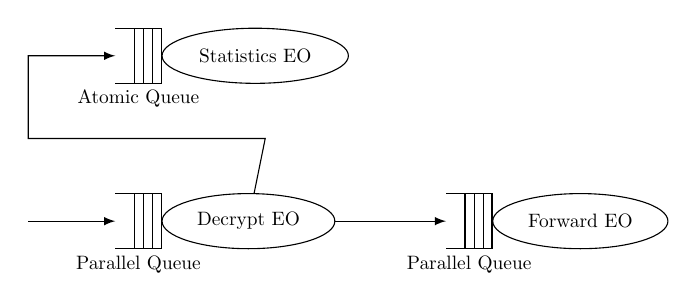
\begin{tikzpicture}[>=latex,node distance=0pt, scale=0.7, every node/.style={transform shape}]
    % the rectangular shape with vertical lines
    \node[rectangle split, rectangle split parts=6,
    draw, rectangle split horizontal,text height=0.5cm,text depth=0.5cm,inner sep=0pt, text width=0.0cm] (parallel1) {};
    \fill[white] ([xshift=-\pgflinewidth,yshift=-\pgflinewidth]parallel1.north west) rectangle ([xshift=-5pt,yshift=\pgflinewidth]parallel1.south);

    \node[draw,ellipse,right= 0pt of parallel1,minimum height=1.0cm,inner xsep=5pt] (decryptEO) {Decrypt EO};

    \node at (6, 0)[rectangle split, rectangle split parts=6,
    draw, rectangle split horizontal,text height=0.5cm,text depth=0.5cm,inner sep=0pt, text width=0.0cm ] (parallel2) {};
    \fill[white] ([xshift=-\pgflinewidth,yshift=-\pgflinewidth]parallel2.north west) rectangle ([xshift=-5pt,yshift=\pgflinewidth]parallel2.south);

    \node[draw,ellipse,right= 0pt of parallel2,minimum height=1.0cm,inner xsep=5pt] (fwdEO) {Forward EO};

    \node at (0, 3)[rectangle split, rectangle split parts=6,
    draw, rectangle split horizontal,text height=0.5cm,text depth=0.5cm,inner sep=0pt, text width=0.0cm] (atomic) {};
    \fill[white] ([xshift=-\pgflinewidth,yshift=-\pgflinewidth]atomic.north west) rectangle ([xshift=-5pt,yshift=\pgflinewidth]atomic.south);

    \node[draw,ellipse,right= 0pt of atomic,minimum height=1.0cm,inner xsep=5pt] (statsEO) {Statistics EO};

    % the arrows and labels
    \draw [->](decryptEO) to (parallel2);
    \draw [->](decryptEO) to (2.3, 1.5) to (-2, 1.5) to (-2, 3) to (atomic);
    \draw [->](-2,0) to (parallel1);

    \node[align=center,below] at (parallel1.south) {Parallel Queue};
    \node[align=center,below] at (parallel2.south) {Parallel Queue};
    \node[align=center,below] at (atomic.south) {Atomic Queue};
\end{tikzpicture}

        \caption{The OpenEM packet processing application.}
        \label{fig:openem-example-flow}
    \end{center}
\end{figure}
An abstract example of a network packet processing application demonstrating the key capabilities of the OpenEM framework is presented in this subsection. In a network packet processing application, network packets are received and transmitted at variable intervals. The example application has to perform some actions for every received packet and decide if the packet has to be forwarded. When a packet is received it is moved into memory accessible by the processor executing the packet processing application and the application is notified of its arrival. The notification is handled by generating an event corresponding to the packet and enqueueing it in the first queue of the application. The event is generated in either hardware or software depending on the OpenEM implementation. A schematic of the queues, execution objects and the connections between them is presented in figure~\ref{fig:openem-example-flow}

The queues of the application may be atomic or parallel. For this example the first queue is parallel. The events in the parallel queue may be scheduled on any core not executing an event currently. The scheduler adheres to the scheduling rules and its optimization parameters, trying to minimize the need to move execution objects from one core to another. The execution object the parallel queue is connected to decrypts the packet contents, which can be done in parallel for many packets at once. After decryption of the packet contents, the execution object decides if the packet needs to be forwarded or dropped. If the packet is forwarded the event is passed forward to a parallel queue connected to another execution object. The second execution object updates the network packet headers and sends it forward. If the packet is dropped, the first execution object frees the event, otherwise it is freed by the second execution object.

The application keeps statistics about the number of packets decrypted, dropped, and forwarded. Since the tasks the statistics are collected for can be done in parallel, the statistics need to be updated in a thread-safe context. To avoid the use of locks in the application code the statistics events are sent to an atomic queue by the first execution object. The atomic queue is connected to the execution object that accesses the shared memory to update the statistics. The update execution object frees the statistics events after it has finished the update.

\section[Texas Instruments Implementation of OpenEM]{Texas Instruments Implementation\\of OpenEM}
\label{sec:tiopenem}
Texas Instruments (TI) provides an implementation of the OpenEM framework for its Keystone I family of multi-core digital signal processors. The OpenEM programming model is suitable for developing DSP applications that utilize the multiple cores of the DSP as well as the various accelerators available. There are many multi-core runtime systems available for multi-core DSPs, including embedded operating systems and operating system agnostic frameworks such as OpenMP. According to TI, the motivation for introducing OpenEM for their multi-core DSPs is that the existing options are not designed for heterogeneous platforms and lack support for features that are often required in DSP applications such as real time constraints~\cite{moerman2014open}.

The TI OpenEM library is delivered as a part of the TI Multicore Software Development Kit (MCSDK), which is available for download at \cite{mcsdkdown}. MCSDK distribution contains source files for the OpenEM components defined in the OpenEM API but no source code is available for the scheduler. In the TI implementation of OpenEM all of the cores run an identical runtime component, which implements most of the framework functionality. The scheduler is not part not part of this component. The scheduler is deployed on a separate PDSP core.

This section describes the Texas Instruments OpenEM implementation version 1.0.0.2. The features specific to the TI implementation of the OpenEM framework are presented in the subsections \ref{subsec:ti-scheduling} Scheduling, \ref{subsec:ti-preloading} Event Preloading, \ref{subsec:ti-acceleration} Hardware Acceleration, \ref{subsec:ti-cache-coherency} Cache Coherency and \ref{subsec:ti-tracing} Tracing. After the descriptions of the features, a look at programming with the TI OpenEM framework is taken in \ref{subsec:ti-init-layer}. Finally the state of the TI OpenEM implementation is examined in \ref{subsec:ti-implementation-state}.

\subsection{Scheduling}
\label{subsec:ti-scheduling}
The TI OpenEM implementation follows the scheduling rules defined by the general OpenEM queue properties as explained in \ref{subsec:queues} and \ref{subsec:schedule}. In addition to the scheduling criteria defined by the OpenEM framework, the TI OpenEM scheduler considers the execution locality. Locality criterion means that the scheduler tries to schedule events so that the cores can execute the same execution object consecutively as much as possible.~\cite{moerman2014open} In DSP applications context switching between execution objects may become expensive if, for example, the program cache does not fit both the execution object ending its execution on the core and the execution object to replace it. By considering locality the scheduler may decrease the overhead caused by the context switching.

The Texas Instruments OpenEM documentation specifies two alternative scheduling modes, namely synchronous and asynchronous scheduling. The asynchronous scheduler is deployed on one of the PDSP cores of the Multicore Navigator described in \ref{subsec:multicorenav}. Scheduling requests sent by the c66x cores described in \ref{subsec:c66x} trigger the scheduling operations of the asynchronous scheduler, but the actual event selection is performed on the PDSP core. The synchronous scheduler is deployed on the c66x cores. The synchronous scheduler interleaves performing the scheduling decisions with executing the execution objects. The synchronous scheduler is not available in the TI OpenEM version 1.0.0.2.~\cite{moerman2014open}

The part of the framework responsible for scheduling consists of two parts: the scheduler and the dispatcher as explained in \ref{subsec:schedule}. The dispatcher is deployed on the c66x cores. The dispatcher checks if there are events scheduled for execution on the core it was called from. The calls to the dispatcher are non-blocking and are made from the application code, typically from within a dispatch loop. The dispatcher returns immediately if no events are available for dispatching. If an event is available the dispatcher will call the receive function of the execution object connected to the queue the event was received from.~\cite{moerman2014open}

\subsection{Event Pre-loading}
\label{subsec:ti-preloading}
The global event buffers, containing the event payload are located in the shared memory of the device. The buffers can be located in the MSMC RAM or in the DDR RAM depending on the space requirements of the buffers. If the event buffer resides in the shared memory when the event has been dispatched, reading the buffer will require accessing the shared memory, which will cause read stalls. Using event pre-loading can minimize these stalls in the TI OpenEM implementation.~\cite{moerman2014open}

Event pre-loading means that moving the event buffers to a core local L1 or L2 memory is started before the event has been dispatched. When an event with event pre-loading enabled is scheduled, one of the Packet DMA engines of the Multicore Navigator will begin to move the event buffers to the local memory. Event pre-loading is enabled separately for every event by the user.~\cite{moerman2014open}

\subsection[Hardware Acceleration in Texas Instruments OpenEM]{Hardware Acceleration in Texas \\ Instruments OpenEM}
\label{subsec:ti-acceleration}
TI OpenEM utilises Multicore Navigator extensively for the scheduler and inter-core communication. Multicore Navigator consists of features that enable hardware accelerated communication between the on-chip devices, including hardware queues and separate cores for queue management. It is described more detail in \ref{subsec:multicorenav}.

The main hardware components used by the OpenEM framework apart from the DSP cores and the different types of memory available, are the hardware queues and one of the PDSP cores of the Multicore Navigator. The hardware queues are used for implementing the software queues of the OpenEM framework. The exact mapping of the software queues to the hardware queues is not documented. The asynchronous scheduler is run on one of the PDSP cores. OpenEM does not use all of the Multicore Navigator queues or PDSP cores, leaving some of the Multicore Navigator resources are available for the user. TI OpenEM provides a mechanism in the framework initialization to divide the Multicore Navigator resources between the application and the framework.~\cite{openemuser}

In OpenEM applications the computational work is done in the execution objects. The execution objects are always deployed on the DSP cores, but they may distribute parts of the communication on hardware accelerators as well. Deeper interaction of the OpenEM application and the hardware accelerators is possible with certain devices that support interfacing with Multicore Navigator. These hardware devices may produce and consume events without software intervention.~\cite{moerman2014open}

The initialization of the OpenEM framework and the required hardware components is handled by the software abstraction layer provided with the example application in~\cite{openemuser}. The software abstraction layer is the best source of information for details about the use of hardware accelerators in OpenEM.

\subsection{Cache Coherency}
\label{subsec:ti-cache-coherency}
The Keystone DSP devices support caching of data in the higher levels of memory to the L1 and L2 local memories but they do not have hardware support for cache coherency \cite{openemapi}. In the general case the application programmer is responsible for managing the cache coherency of the application. TI OpenEM provides optional automatic cache coherency management for event buffers. The cache coherency mode can be set for each event individually. Automatic coherency management is also partially supported for queue contexts.~\cite{moerman2014open}

\subsection{OpenEM Tracing}
\label{subsec:ti-tracing}
TI OpenEM includes a built-in tracing feature that provides data about the runtime behaviour. The trace API is simple to use. The application has to register a trace handler with the OpenEM runtime and link the application with a trace-enabled version of the runtime library.~\cite{openemapi}

The trace handler will be called every time the runtime or the application makes calls to OpenEM functions and it will be passed information about the type of the call made. The programmer should note that multiple cores may call the handler at overlapping times and therefore race conditions are possible.~\cite{openemapi} Tracing can be used for example to track the number of events in each queue. This type of tracking may help debug problems with congestion and many other types of problems with OpenEM.

\subsection{Programming with TI OpenEM}
\label{subsec:ti-init-layer}
The OpenEM framework was not designed by NSN to be a full software platform or a middleware solution as explained in the OpenEM design principles available at \cite{openempage}, which are reproduced in \ref{sec:emframework}. However the level of abstraction is suitable for DSP programming, which is done close to the hardware without an operating system. The low abstraction level means that the developer using TI OpenEM for developing applications for DSPs has to pay attention to the hardware initialization, memory allocation and cache coherency for their own code as well as for the framework.~\cite{openemuser}

The hardware initialization required by TI OpenEM is implemented in the example application described in \cite{openemuser}. The initialization code is not a part of the OpenEM framework, but the initialization code provided in the example application works without modification or with minor modifications for most purposes. The initialization layer provides an API for coordinating the hardware resource use between the application and the framework. \cite{openemuser} The framework initialization documentation is incomplete and the application developer has to look at the source code of the example initialization layer to find out about the resource use of the framework if there exists a possibility of conflicting use.

\subsection{State of TI OpenEM Implementation}
\label{subsec:ti-implementation-state}
The TI OpenEM library version 1.0.0.2 does not implement the complete OpenEM API as specified by the NSN implementation of OpenEM described in \ref{sec:emframework}. The following listing presents the unimplemented features as listed in the OpenEM library version 1.0.0.2 release notes \cite{openemnotes} and the TI OpenEM white paper \cite{moerman2014open}.

\begin{itemize}
    \item \textbf{Event Groups},
        The TI implementation of event groups is functional but lacks the functionality to delete event groups.
    \item \textbf{Distributed Scheduling},
        A synchronous scheduler is described in \cite{moerman2014open}. Distributed Scheduling is not part of the NSN specification of OpenEM.
    \item \textbf{Co-operative dispatcher},
        The co-operative dispatcher is described in \cite{moerman2014open} provides services for suspending and resuming events. The co-operative dispatcher only works with the synchronous scheduler.
    \item \textbf{Execution Object context}
    \item \textbf{Parallel Ordered Queue}
    \item \textbf{Unscheduled Queue}
\end{itemize}

In addition to the limitations listed above the Queue Group implementation appears incomplete in the version 1.0.0.2. Queue Groups can be defined and modified as described in \ref{subsec:queues} but only one queue group can exist at a time. This could be a limitation of the hardware platform but there is no mention of the limitation in the TI OpenEM implementation documentation or the header files.

\chapter{Multi-core DSP in Video Stream Processing}
\label{chapter:experiments}
The objective of this thesis is to understand the performance of the Texas Instruments implementation of Open Event Machine in stream processing. The objective is achieved by implementing a video stream processing application using OpenEM, measuring its performance and comparing that to a comparable, statically scheduled application. The comparable application is implemented using the PREESM framework. Both of the applications are instrumented in similar manner.

In this chapter the material and methods used in the experiment are introduced. The performance and behavior of OpenEM is evaluated using quantitative analysis. The analysis methods are explained in section \ref{sec:performance-analysis}. The hardware platform used in the experiments is the Texas Instruments TMS320C6678, which is described in \ref{sec:c6678}. PREESM provides the tools for implementing the comparable workload. PREESM is introduced in section \ref{sec:preesm}. The workload application processes video streams. An overview to video streams is provided in section \ref{sec:video-streams}. Finally, the algorithms computed in the stream processing application are part of the Canny edge detection algorithm introduced in \ref{sec:canny}.

\section{Performance Analysis}
\label{sec:performance-analysis}
To understand the behavior and performance of software systems, quantitative data about the system execution is required. Precisely what data is needed depends on the purpose of the analysis. A couple of popular methods for acquiring quantitative data about software systems are introduced in this section. First, an overview to the performance analysis of software systems is provided in the subsection \ref{subsec:analysing-software}. Second, a closer focus to measuring software systems is taken in subsection \ref{subsec:measuring-software}. Finally, the analysis of the acquired data is described in subsection \ref{subsec:data-analysis}.

\subsection{Analysing Software Systems}
\label{subsec:analysing-software}
According to Jain \cite{jain1991art} the performance analysis of software systems can be split into three categories, which are analytical modeling, simulation and measuring of software systems. Analytical modeling and simulation use mathematical models for the analysis of the software systems. Abstract mathematical models of a system can be constructed without access to the system under study. To measure a software system, access to the specific system under study is always required. There are many methods for modeling and simulation of software systems, but in most cases they require less work to implement than the actual system under study. These properties make the analytical modeling and simulation attractive for explorative study of software systems that do not exist yet.~\cite{jain1991art}

The key difference between analytical modeling and simulation is the notion of time present in simulation. Analytical modeling solves the system state at a fixed point in time, in contrast to simulators where the system state is computed iteratively at multiple points in time.~\cite{jain1991art}

Performance analysis is used for many different purposes. For example performance analysis can be used to help choose the best performing hardware platform for certain application, or to explore different configurations of an application. Successful analysis requires careful experiment design. First step to successful performance analysis is method selection. Using simulation or analytical modeling can yield results quickly, but they are not as accurate as measuring the real world system.~\cite{jain1991art}

The execution of a computer program is a complex interaction of hardware and software components and thus the number of parameters of the analysis grows large. Factors are parameters that are varied in the analysis. Factors are selected from among all parameters of the system \cite{jain1991art}. Every factor increases the time it takes to complete the analysis and only few of the parameters are relevant for the result of the analysis. Thus, the factor selection requires clear goals for the analysis and a good understanding of the problem space so that the most relevant factors are chosen. The factor selection of the experiments conducted in this thesis is discussed in section \ref{subsec:parameters-and-factors}.

\subsection{Measuring Software Systems}
\label{subsec:measuring-software}
In this thesis a measurement system consisting of a workload, applications and execution hardware is constructed and its performance is measured. In this subsection a closer look at measuring software systems is taken.

The successful comparison of software systems requires meaningful and reasonably accurate measurements of the systems under study. Measurements are obtained by monitoring the system while it is being subjected to a particular workload \cite{jain1991art}. Often the monitored applications are built for the comparison purpose only and therefore any workload they are subjected to is an approximation of the real world workload that would be processed by their real world application counterparts. These approximate workloads are called synthetic workloads. The use of a synthetic workload gives more control over the test conditions and most importantly makes the experiments repeatable.~\cite{jain1991art}

Synthetic workload creation requires care because it needs to mimic its real world counterpart with high accuracy to provide useful any information. Performance analysis is often conducted to understand the performance or feasibility of a software component or a system that does not exist yet. In such situations synthetic workloads need to be used out of necessity.  

The workload is the target of the measurements but it does not define the exact measurements that are to be conducted. Selection of metrics is equally important as the selection of the workload for successful analysis. The best metrics for a given analysis are determined by what is the goal of the analysis. \cite{jain1991art} For example measurements can be used for comparison of throughput of two comparable software systems. In that case clearly a good measure of throughput is needed.

The software measurement tools are called monitors, which can be implemented both in hardware and in software. Monitors are classified to software monitors, hardware monitors, firmware monitors or hybrid monitors depending on the implementation level of the monitor. The implementation level of the monitor affects the level of events that are convenient to measure with it. For example hardware monitors can monitor the state of registers and hardware counters but have difficulties in observing the status of software constructs such as the execution of functions. The software monitors on the other hand can be used to monitor the status of software components but gathering information about the status of the hardware is more difficult and in some cases impossible. \cite{jain1991art} For example it is very complicated to determine whether a memory operation hit a given level of cache or not using software alone but many hardware platforms offer hardware counters to monitor the cache hits and misses.

\subsection{Analysis of the Measurement Data}
\label{subsec:data-analysis}
The goal of the performance analysis is to get actionable results about the systems under study. The data obtained from the models or measurements is not in itself enough for making well-grounded decisions. The models and measurements may yield millions of values for the observed variables and the analyst needs to decide how to best represent the data so that the phenomena behind the data are explained \cite{jain1991art}.

Statistical methods are used to analyze the numerical data and expose the causation and correlation between the factors and the results. Often in the literature simple statistical tools such as mean, mode and standard deviation are used to represent the data in only a few numbers. Such simple statistics are enough if they capture the relevant information about behavior of the system. For example if the goal of the analysis is to compare the latency of two non-realtime systems, an average of the latency and its standard deviation over a reasonable measurement period can be enough. A more thorough look at the statistical tools is provided in \cite{jain1991art}.

The results of the analysis are often easiest to understand when presented in graphical form. Graphical representations of the data such as histograms, line charts and bar charts are commonly used. These graphs are very generic and used in many fields to present many kinds of data. There are also more domain specific visualizations of data such as the Gantt charts used to represent schedules in computer context and elsewhere. The visualizations of data are designed to be faster to understand than the corresponding numerical views to the same data but they have their limitations. The graphical representations are inaccurate and if they are not carefully prepared they may present a biased view to the real data. Due to these limitations the visualizations should be prepared carefully and the numerical data they are based on should be also made available.~\cite{jain1991art}

\section[Texas Instruments TMS320C6678]{Texas Instruments\\TMS320C6678}
\label{sec:c6678}
This section describes the hardware platform used in the experiments. The experiments were conducted on a Texas Instruments TMS320C6678 multi-core digital signal processor. First, the selection of the TMS320C6678 as the hardware platform for the experiments in this thesis is explained in subsection~\ref{subsec:selection-of-platform}. Second, an overview of the hardware platform is given in subsection~\ref{subsec:hw-overview}. After the overview, the key features of the platform are described in subsections \ref{subsec:c66x} C66x DSP, \ref{subsec:c66memory} Memory Hierarchy and \ref{subsec:multicorenav} Multicore Navigator.

\subsection{Selection of the Hardware Platform}
\label{subsec:selection-of-platform}
This thesis investigates stream processing with Open Event Machine on a multi-core DSP. The Texas Instruments Keystone I family of multi-core DSPs has an advanced support for multi-core programming, including a Texas Instruments implementation of OpenEM~\cite{MCSDKbrochure}. The multi-core programming support has not always been a design priority of multi-core DSPs, for example the TMS320C647x DSPs were looked at as, "multiple single-core DSP in a single package" by the programmers~\cite{moerman2014open}.

The hardware platform used in the experiments in this thesis is the Texas Instrument TMS320C6678. The TMS320C6678 is a fixed and floating point digital signal processor based on the Texas Instruments Keystone I architecture~\cite{tmsdatasheet}. The Keystone I architecture was selected because there exists an OpenEM implementation for that supports the processors implementing the architecture. Out of the Keystone I devices TMS320C6678 was selected because Advantech provides an evaluation module TMDXEVM6678L for the specific processor, which makes the experimentation more straightforward than building an evaluation platform from scratch. Another benefit of the TMS320C6678 is that the PREESM rapid prototyping tool for dataflow applications has support for it~\cite{pelcat2014preesm}.

\subsection{TMS320C6678 Overview}
\label{subsec:hw-overview}

\begin{figure}[h!]
    \begin{center}
        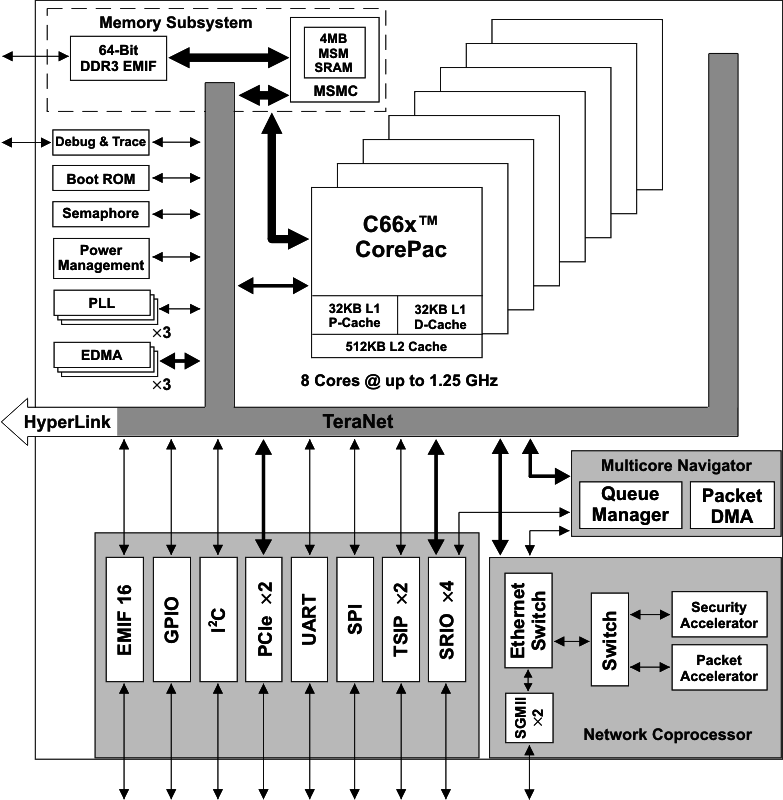
\includegraphics[width=0.99\textwidth]{images/fbd_SPRS691e.png}
        \caption{High-level schematic of the TMS320C6678 architecture. Figure from~\cite{tmsdatasheet}.}
        \label{fig:arch_overview}
    \end{center}
\end{figure}

The TMS320C6678 is based on the Keystone I architecture. The Keystone I architecture specifies a set of hardware elements which enable integration of C66x DSP cores, application specific co-processors and IO \cite{tmsdatasheet}. The Keystone I hardware modules and their connections are presented in the figure \ref{fig:arch_overview}. The points of interest in the figure in the scope of this thesis are the C66x CorePac cores depicted in the middle of the figure, the memory subsystems and its components in the top-left of the figure and the Multicore Navigator depicted in the right edge of the figure.

In the Keystone I architecture there are multiple ways for the C66x cores to communicate with each other, the memory and the peripherals. The methods of communication of specific interest for the experiments in this thesis are communication through shared memory discussed in subsection \ref{subsec:c66memory} and communication through packet based communication manager Multicore Navigator introduced in subsection \ref{subsec:multicorenav}.

The development board used for development of the experiment applications and measurements is an Advantech TMDXEVM6678L. The board is an evaluation module for the TMS320C6678 multi-core DSP. The evaluation module has 512 megabytes of DDR3 memory which is sufficient for stream processing applications. Another important feature of the evaluation module is the emulator module with USB connectivity. The emulator together with the Code Composer Studio IDE (CCS) make the programming and debugging the experiment programs for the DSPs uncomplicated.~\cite{evmref} CCS version 5.2 is distributed with the hardware evaluation module and was used for development of the experiments in this thesis.

\subsection{C66x DSP}
\label{subsec:c66x}
The hardware platform used in this thesis is the TMS320C6678 multi-core digital signal processor. The processor consists of eight C66x DSP cores. The C66x is based on the Texas Instruments TMS320C66x instruction set architecture. The TMS320C66x is a very long instruction word architecture, which allows for high amount of instruction level parallelism. The C66x has a total of eight functional units, which operate in parallel. This means that the C66x can dispatch up to eight instructions per cycle. The instructions dispatched in parallel move through pipeline stages simultaneously. Pipelining helps eliminate CPU stalls while waiting for memory operations or other CPU instructions taking multiple cycles complete.~\cite{sprugh7}

Keeping the utilization of the wide pipeline high, the CPU needs to have enough registers to prevent excessive memory access stalling. The CPU has 64 32-bit general purpose registers~\cite{sprugh7}. The C66x is a high-end processor with native support for 32-bit and 64-bit floating point instructions and capability of clock speeds up to 1.4 GHz~\cite{sprugh7}.

\subsection{Memory Hierarchy}
\label{subsec:c66memory}
The TMS320C6678 contains a multi-layer memory hierarchy which can be configured by the user to a large extent. The memory hierarchy in the device consists of L1 and L2 memories for each core, Multicore Shared Memory (MSM) and additionally external memory provided by the evaluation module. In the figure~\ref{fig:arch_overview} the memories are placed inside the subsystems they are part of, MSM can be found in the upper-left corner as part of the memory subsystem.

Each c66x CPU has 32 KB level 1 program cache (L1P), 32 KB level 1 data cache (L1D). Each CPU also has 512 KB of level 2 cache. Both of the L1 caches and the L2 cache can be found in the figure~\ref{fig:arch_overview} as part of the C66x CorePac box. Initially after bootup both L1P and L1D are configured as cache but they can be reconfigured as addressable memory by software. The L2 memory is always configured as addressable memory after reset but can be configured as cache by software. \cite{tmsdatasheet} L2 SRAM addresses are always cached with L1P and L1D whereas external memory addresses are configured noncacheable by default~\cite{cacheguide}.

Configuring the state of the L1 and L2 memories as well as other memory configurations can be handled with software \cite{sprugh7}. CCS automatically handles a lot of the memory mapping needed for applications and provides tools for creating custom configurations.

In PC hardware cache coherence is usually handled automatically by the hardware. In c66x, however, that is not the case. Each c66x core maintains cache coherence between its L1 caches and the L2 cache automatically but programmer needs to manage coherence in most other cases. For example if caching is enabled for an external memory region shared by two cores, explicit cache coherence operations need to be performed before each core can read from or write to the shared region~\cite{cacheguide}.

The evaluation module has 512 MB of DDR3 memory \cite{evmref}. The memory in the evaluation module, as any external memory in other hardware configurations, is accessible through the Multicore Shared Memory Controller (MSMC). The MSMC itself contains 4096KB of shared memory accesible by all cores. In the figure~\ref{fig:arch_overview} the memory subsystem contains the EMIF link to the external memory and the MSMC.

\subsection{Multicore Navigator}
\label{subsec:multicorenav}
The multi-core programmability of the TMS320C6678 makes it interesting for this thesis. The device is designed to allow simple co-operation of the DSP cores and provides the required hardware support for that purpose. The core features enabling the multi-core programmability are grouped under the name of Multicore Navigator.

Multicore Navigator is the name for a collection of features in Keystone I and II devices, which enables hardware-accelerated, packet-based communication between on-chip devices. Texas Instruments claims the use of specialized hardware for on-chip communication results in significant performance gains when implemented carefully. The design goals stated for the Multicore Navigator in \cite{navigator} are minimizing host interaction and maximizing memory use efficiency.~\cite{navigator}

In Keystone I devices such as the TMS320C6678, the Multicore Navigator provides a hardware queue manager, a special direct memory access for different subsystems called Packet DMA (PKTDMA), and multi-core host notifications via interrupts. \cite{navigator} The Texas Instruments OpenEM implementation \ref{chapter:openem} heavily utilizes the features provided by Multicore Navigator.

The Queue Manager on Keystone I architecture devices is a hardware module that manages 8192 queues. Packets are queued and dequeued from the queues by the applications. The Queue Manager is responsible for accelerating the packet communication. In addition to the Queue Manager the Queue Management Subsystem contains two Packed Data Structure Processors (PSDP) which perform tasks related to the queue management and packet communication. For example the PDSP processors can be used to perform accumulation of packets. The accumulation program is given a list of queues to poll. Whenever it finds a descriptor from one of the queues it is watching it will pop the descriptor and place it in a buffer provided by the application. After a pre-determined number of descriptors, or after reaching its time limit, the accumulator program notifies the host processor about the descriptors in the buffer via an interrupt. Use of such firmware offloads the burden of queue polling from the host processors.~\cite{navigator} The TI implementation of OpenEM \ref{chapter:openem} provides its own firmware for the PDSP cores which is utilized by the OpenEM runtime for event scheduling \cite{moerman2014open}.

The PKTDMA is a special DMA utilized by the Multicore Navigator to transfer packet buffers between memory locations. When a packet is sent to a queue The PKTDMA reads the address of the data to be transferred from packet descriptor, transfers the data in one or more data moves and writes the pointer to the data queue specified as the receiver of the packet. The PKTDMA is useful because it allows the program running on a PDSP core to move data in the memory without interrupting the host processors.~\cite{navigator} OpenEM uses PKTDMA to move event buffers to the caches of the core, which is about to receive the event~\cite{moerman2014open}.

\section{PREESM}
\label{sec:preesm}
PREESM is a rapid prototyping framework for multi-core development. For understanding the OpenEM framework a way to construct comparable programs with statically scheduled multi-core runtime was needed. PREESM provides a way to quickly construct multi-core applications for PC as well as for the Texas Instruments multi-core DSP used in the experiments. In this chapter the PREESM framework is introduced. First, an overview of the framework is given in subsection \ref{subsec:preesm-overview}. Second, the framework overview, the internal representations used by the framework are described in subsection \ref{subsec:preesm-internal}. Third, scheduling in the PREESM framework is explained in section \ref{sec:preesm-scheduling}. And finally, the memory allocation and code generation in PREESM are explained in section~\ref{sec:preesm-codegen}.

\subsection{PREESM Overview}
\label{subsec:preesm-overview}
PREESM is a collection of tools for rapid prototyping multi-core applications. The tools include a graphical editor for the hardware and the software models, code generators for multiple hardware platforms and an automated generator for fixed schedules. The PREESM tools are used through the Eclipse IDE based environment available at~\cite{preesm}.

In PREESM prototypes of applications are constructed by combining hardware and software models with manually created source code and automatically generated schedule. The software model used in PREESM is based on dataflow models of computation and it is discussed in detail in subsection \ref{subsec:preesm-internal}. To create a software model in PREESM the application is divided into actors. The actors contain manually created code, which is often written in side-effect free style to enable parallel execution of the actors, but this is not enforced by the framework. The graphical editor for the software model allows the user to create actors and connect them together using first in first out queues.~\cite{preesm}

The model of the target hardware platform is created using a similar graphical tool as the software model. The hardware model is described in subsection \ref{subsec:preesm-internal}. PREESM parses the graphs of the models and creates a static schedule for the executable. The schedule, the actor implementations and the graphs are inputs for the code generator, which creates the multi-core executable.~\cite{pelcat2014preesm} The graphical tools allow the PREESM user to create dependencies between the actors. They also allow a more fine grained control over the code generation by setting estimated actor execution times and selecting the cores on which each actor is allowed to execute.

\begin{figure}[h!]
    \begin{center}
        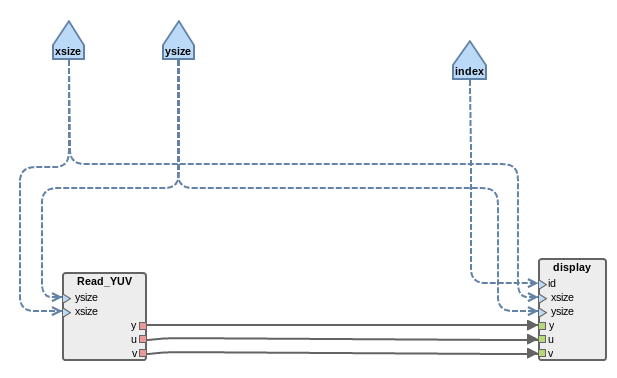
\includegraphics[width=0.99\textwidth]{images/example_preesm_diagram.png}
        \caption{A simple dataflow diagram created with PREESM.}
        \label{fig:preesm_example}
    \end{center}
\end{figure}

\subsection{PREESM Internal Representations}
\label{subsec:preesm-internal}
PREESM applications are created by combining inputs of two different internal representations and manually created source code. The PREESM internal representations are described in this subsection. First, a look is taken at the PREESM algorithm representation PiSDF and second, to the PREESM hardware model.

In PREESM the applications are modeled using a synchronous dataflow based representation of the software called parameterized and interfaced synchronous dataflow model of computation (PiSDF)~\cite{pelcat2014preesm}. PREESM provides graphical tools for editing the dataflow diagram. An example of an dataflow diagram created in PREESM is presented in figure \ref{fig:preesm_example}. The biggest benefit of using synchronous dataflow based model of computation is that deadlock free static schedules can be generated from them~\cite{pelcat2014preesm}. The static schedules generated by PREESM are guaranteed to be deadlock free~\cite{preesm}.

PREESM uses an extended version of SDF called PiSDF \cite{pelcat2014preesm}. PiSDF extends SDF by providing hierarchical graphs based on interfaces and by introducing parameterized actors. An actor in PiSDF can be replaced by a subgraph, which has input and output interfaces. The interfaces insulate the hierarchy levels in terms of schedulability analysis, meaning that schedules can be generated for the subgraphs without knowledge of the higher level models. The parameters are used to configure the production and consumption rates of the actors.~\cite{desnos2013pimm}

An example of a PiSDF graph is presented in figure \ref{fig:preesm_example}. The parameters of the PiSDF model are presented at the top of the figure as pentagons connected to the actors with dashed lines. The actors have input and output ports for parameters and data. The ports define the input and output interfaces of the actors. The actual data paths are the arcs connecting the actors in the bottom of the figure.

The PREESM code generation is aware of the target hardware platform. PREESM uses an internal representation called the System-Level Architecture Model (S-LAM) \cite{pelcat2009system} to describe the target architecture. S-LAM is designed specifically to provide architecture models of high abstraction level for rapid prototyping purposes. S-LAM has good expressive power and it is suitable for modeling heterogeneous architectures as a S-LAM can contain different types of computational resources and communication links.~\cite{pelcat2009system} In the PREESM context however, the typical S-LAM models are simple. For example the S-LAM representing the TMS320C6678 used in experiment \ref{subsec:first-experiment} is quite simple consisting of eight c6678 cores connected through shared memory.

In PREESM the user inputs the speeds of the hardware components of the S-LAM and the speeds of the connections between them. This information is used by the PREESM scheduler to generate a static schedule, that takes communication delays and the component speeds into account, trying to minimize the time spent waiting for communication.~\cite{pelcat2009system}

\subsection{PREESM Scheduling}
\label{sec:preesm-scheduling}
Scheduling multi-core applications is not a trivial task, because the execution on a single core is sensitive to what other cores are doing. An unsuccessful schedule may result in the application deadlocking or many other kinds of problems. The approach PREESM takes to overcome the complexity of scheduling multi-core applications is using a highly analysable model of computation PiSDF and creating a static schedule based on it. PREESM uses the \textit{List} and \textit{Fast} scheduling methods described in \cite{kwok1997high} for generating a static schedule for multi-core platforms. Using these methods PREESM is able to generate a static schedule and guarantee that it is deadlock free.

The reason why multi-core applications are created in the first place is the performance increase available through parallelizing the execution. To get a performance increase from parallelizing the application the scheduler must be able to efficiently utilize the multiple cores. The critical measure of performance can be throughput or latency. The designer of the PREESM scheduler has made a decision to focus on so-called latency dominated systems \cite{pelcat2014preesm}. Latency dominated system is defined in \cite{ghamarian2006throughput} as a system where respecting the latency constraint placed upon the system automatically guarantees the satisfaction of the throughput constraint. In other words in the systems PREESM is designed for, each iteration of the application has to fulfill some latency constraint. Fulfilling this latency constraint yields satisfactory throughput. This frees the PREESM scheduler from considering throughput in the scheduling decisions and yields a simpler schedule. Because the scheduler only considers the latency of the execution, the iterations of the algorithm are not interleaved. Instead, all cores are synchronized between the iterations with a barrier.~\cite{pelcat2014preesm}

The execution of the different iterations of the algorithm is not interleaved by the PREESM scheduler. However, intra-iteration interleaving is supported. In intra-iteration interleaving the actors belonging to the same iteration of the algorithm are executed in parallel. \cite{pelcat2014preesm} An example of the intra-iteration interleaving is given in the software pipelining tutorial available at \cite{preesm}.

The dependencies between the actors are defined by the PiSDF model of the application. These dependencies are enough to generate ordering of the actor firings, but to get an efficient schedule the execution times of the actors are needed. The estimated execution times for each actor are provided by the user. The time required for communication between the actors is approximated from the amount out data to be transferred and the speed of the communication links. The data amounts are defined in the actor model and the communication speeds in the S-LAM. With the actor ordering and the timing information, the framework generates a static schedule. \cite{pelcat2014preesm} PREESM framework visualizes the generated schedule with a Gantt chart. An example Gantt chart is presented in figure \ref{fig:preesm_gantt}.

\subsection{PREESM Memory Allocation}
\label{sec:preesm-codegen}
The output of the PREESM framework is a multi-core executable. Before the schedule and the user created actors can be combined into an executable, PREESM has to determine how much memory is required for the communication between the actors. The size of every data transfer is determined by the input and output interfaces of the actors and it does not change during the execution. Because the size of the buffers is static, the buffers can be allocated before the execution.~\cite{desnos2012memory}

The data in the communication buffer is considered reserved from the beginning of the execution of the producing actor to the end of execution of the consuming actor. This choice is made to enable custom production rates of the actors. Due to this choice the actors cannot reuse their input buffers as their output buffers. \cite{desnos2012memory} This approach keeps the resulting executable simple but it results in extra copying of buffers between the actors.

In the simple case where the producing and the consuming actors execute on the same core and are not dependent on any other actors, simple copying of buffers is enough. However when the producing actor executes on a different core than the consuming actor, the cores need to synchronize before the consuming actor can start to execute. If the user provided estimates for the execution times of the actors are accurate, the synchronizations should not cause a lot of waiting.~\cite{pelcat2014preesm}

With the memory allocations computed, the framework can create an executable. The structure of the complete application follows the template provided by the framework. The memory allocations are handled in the initialization. After the initialization the cores enter loops where the static schedule for each core is laid out as interleaved calls to actor implementations, memory operations to move the data between the buffers and synchronization barriers.

\section{Video Streams}
\label{sec:video-streams}
Many different video stream formats are needed to capture, transfer and store videos. Raw video material requires a lot of space to store and a lot of bandwidth to transfer but when the video data is edited, the part of the video stream that is being edited has to be in unpacked format. In this section two standards related to video streams are explained. First the YUV color specification and second the CIF frame resolution format.

\subsection{YUV Format}
\label{subsec:yuv}
YUV color space is used in encoding colors of images and videos. The YUV color system is used for example in encoding the colors of television broadcasts using the PAL or NTSC systems. The YUV color space is designed with the human perception in mind, meaning the channels are selected so that compression artifacts and other errors are more likely masked by human perception. This allows for reduced bandwith compared to RGB encoded colors. The Y channel corresponds to the luminance of the image. Luminance means the perceived brightness. In a black and white image or video only the Y channel is used. The U and V channels are called the chrominance channels and they encode the color component of the image.~\cite{jack2011video}

In digital media YUV term is commonly used to refer to YCbCr, which is a way of encoding RGB color information. Y' (Y prime) is called luma and is distinct from the Y channel of the analog YUV system. The luma channel is a non-linear encoding of the light intensity. Cb and Cr are the blue-difference and red-difference components respectively. It is common to store the luma channel at a higher resolution than the chroma channels to save bandwidth. This process is called chroma sub-sampling. Humans are more sensitive to the brightness of the image than the color of the image and thus the lower resolution of the chroma channels causes less noticeable artifacts.~\cite{jack2011video}

\subsection{Common Intermediate Format}
\label{subsec:cif}
Common Intermediate Format or CIF is a standardization of the horizontal and vertical resolutions of pixels in video signals. The CIF pixels are non-square with an aspect ratio of approximately 1.222:1. The standard defines multiple resolutions such as the CIF 352x288 and QCIF for quarter CIF 176x144.CIF resolutions were designed to be easily convertible to the PAL and NTSC systems.~\cite{telecommunication1993itu}

\section{Canny edge detector}
\label{sec:canny}
Edge detection is an important tool in image processing and computer vision. Many image processing and computer vision algorithms operate on detected edges. The quality of the detected edges is important for the algorithms using them as input. In his 1986 paper John F. Canny \cite{canny1986computational} lays out the mathematical criteria for successful edge detection and presents an algorithm, which achieves decent edge detection performance. The algorithm is suitable for implementation on DSPs. The Canny edge detection algorithm consists of five steps presented in the following list.

\begin{enumerate}
    \item{Noise reduction}
    \item{Finding the intensity gradient of the image}
    \item{Non-maximum suppression}
    \item{Double thresholding}
    \item{Edge tracking by hysteresis}
\end{enumerate}

In the canny edge detector the image is first filtered with a gaussian filter to reduce the amount of noise in the image. Second, the changes in the intensity in the image are detected using an image gradient operator such as the sobel operator. The third step improves the accuracy of the edge detection by suppressing all but the strongest responses to the detected edges, in practice ``thinning'' the edges. The fourth step classifies the edge pixels to three classes separated by empirically determined threshold values. The pixels with gradient value above the high threshold are marked strong pixels and the pixels with gradient value below the low threshold are suppressed. In the fifth step the remaining weak pixels with gradient values below the high threshold are preserved or suppressed according to the presence of strong pixels in their neighborhood. Detailed description of the algorithm is presented in the original paper by Canny \cite{canny1986computational}, information about implementing a canny edge detector is available in \cite{gonzalez2008digital} and comparison of its performance to other edge detectors can be found in \cite{maini2009study}.

In this section the phases of canny edge detector are described in the order they are used in Canny filter. First, the gaussian filter is introduced in subsection \ref{subsec:gauss}. The sobel filter is looked at next in subsection \ref{subsec:sobel}. After the sobel filter, the edge responses are pruned in three phases. The three phases are presented in subsection \ref{subsec:canny-edge-pruning}.

\subsection{Gaussian filter}
\label{subsec:gauss}
Gaussian filtering is used for multiple purposes in digital image processing. In the canny edge detector the gaussian filter is used to reduce noise in the processed images. The gaussian filter works by convolving a gaussian function with the input signal. Gaussian function is non-zero everywhere which means it would theoretically require an infinite convolution window. Since the function decays rapidly it is often reasonable to truncate the function and use small windows.~\cite{gonzalez2008digital} 

Calculating the convolution with a truncated function means in practice that every pixel in the filtered image has an intensity value computed by taking a weighted average of the neighboring pixels in the input image. The weights are pre-calculated from the gaussian function, giving the highest weight to the pixel in the center of the window. The gaussian filter displayed in figure \ref{fig:gaussmat} was calculated with $\sigma$ = 1.3. The filtered image has a smoothed appearance compared to the original image.

\begin{figure}
    \begin{displaymath}
        B = \frac{1}{159}\begin{bmatrix}
             2 & 4 & 5 & 4 & 2 \\
             4 & 9 & 12 & 9 & 4 \\
             5 & 12 & 15 & 12 & 5 \\
             4 & 9 & 12 & 9 & 4 \\
             2 & 4 & 5 & 4 & 2 \\
        \end{bmatrix} \ast A
    \end{displaymath}
    \caption{Convolution with a gaussian kernel computed with $\sigma = 1.3$. The convolution operation is denoted by the asterisk.}
    \label{fig:gaussmat}
\end{figure}

\subsection{Sobel filter}
\label{subsec:sobel}
The actual edge detection in the canny edge detector begins with determining the changes in the intensity of the image. This is done by applying the sobel operator to the input image. The sobel operator is a discrete differentiation operator. It consists of two 3x3 kernels which are convolved with the image to approximate the derivatives. The two kernels represent horizontal and vertical changes. At each point in the image the resulting gradient approximations are combined giving an approximate gradient magnitude. \cite{gonzalez2008digital} The convolution operations are presented in figure \ref{fig:sobelmat}.

\begin{figure}
    \begin{displaymath}
        G_{x} = \begin{bmatrix}
            -1 & 0 & +1 \\
            -2 & 0 & +2 \\
            -1 & 0 & +1 \\
        \end{bmatrix} \ast A
    \end{displaymath}
    \begin{displaymath}
        G_{y} = \begin{bmatrix}
            -1 & -2 & -1 \\
            0 & 0 & 0 \\
            +1 & +2 & +1 \\
        \end{bmatrix} \ast A
    \end{displaymath}
    \caption{The 3x3 Sobel kernels used in the application to compute the gradient approximation. $G_{x}$ is the horizontal gradient approximation at given pixel and $G_{y}$ is the vertical gradient approximation. The asterisk denotes the convolution operation.}
    \label{fig:sobelmat}
\end{figure}

\subsection{Canny Edge Pruning}
\label{subsec:canny-edge-pruning}
Canny edge detector is designed to detect edges accurately and as unambiguously as possible. To make unambiguous detections, each edge in the input image should produce only one edge response. For this purpose Canny edge detector employs \textbf{non-maximum suppression}. Non-maximum suppression works on the gradient image that was calculated in the previous phase. For each pixel in the gradient images, non-maximum suppression compares the gradient value to the adjacent pixels in positive and negative gradient directions. The pixel is preserved only if it has the largest gradient value compared to its neighbors.~\cite{gonzalez2008digital}

The non-maximum suppression outputs an image where the edge responses have been pruned to single response per edge, but there still remain gradient pixels that correspond to noise or other uninteresting variations in the image. The detection quality is further improved by applying two thresholds to the output of the non-maximum suppression phase. In the literature this phase is called \textbf{double thresholding}. If the gradient value of a pixel is higher than the high threshold, the pixel is marked as a strong pixel. If the value is lower than the high threshold but higher than the low threshold, the pixel is marked as weak pixel. Pixels with gradient values lower than the low threshold are automatically discarded. The threshold values are determined empirically.~\cite{gonzalez2008digital}

In the final phase of the Canny edge detector, called \textbf{edge tracking by hysteresis} the strong pixels are used to determine which of the weak pixels to keep and which to discard. A weak pixel is preserved if there is at least one strong pixel among its eight neighboring pixels. If there are no strong pixels in the neighborhood the weak pixel is discarded.~\cite{gonzalez2008digital}

\chapter{Experiment Construction}
\label{chapter:construction}
This chapter describes the implementation of the applications studied in the experiments. The workload application was inspired by Canny filter. Two versions of the workload are implemented and both are instrumented for measurement. Three experiments were designed for comparison of the applications.

To begin this chapter the general idea of the workload application is introduced in~\ref{sec:filterapp}. Then the PREESM implementation of the application is described in~\ref{sec:preesmapp}. Next the OpenEM implementation is explained in~\ref{sec:oemapp}. After the applications have been described, the instrumentation explained in~\ref{sec:instrumentation}. Finally the experiments introduced in~\ref{sec:experiment-description}.

\section{Filter Application}
\label{sec:filterapp}
The objective of this thesis is to study the suitability of OpenEM framework for building stream processing applications. Video streams make up an increasing proportion of the data being transferred in the internet. The processing of video streams requires a lot of computing power, as the streams have increasingly high bitrates and they have to be compressed for transfer and storage. Thus video streams are especially interesting streams to study and were selected as the stream format for the experiments conducted in this thesis.

Three requirements for the workload applications were specified to guide the design. The requirements are presented in the following list.

\begin{enumerate}
    \item{Variable input bitrates}
    \item{Comparability the PREESM and OpenEM applications}
    \item{Highly analyzable}
\end{enumerate}

\textbf{Variable input bitrates} were required of the workload applications to make it possible to study the performance of the OpenEM framework in processing dynamic workloads. Varying the bitrates of the video stream inputs is simple as the frame size of the stream is easy to change and it doesn't affect the algorithms used in any unforeseeable way. \textbf{Comparability of the PREESM and OpenEM applications} was required so the PREESM workload could be used as a baseline implementation. Last requirement for the applications was that they needed to be \textbf{highly analyzable} in order to enable the study of OpenEM performance. An application satisfying these requirements was designed using the PREESM sobel example at \cite{preesmtut} as the starting point and adding another processing component to it. It is important to notice that the actual performance of the filter application in its nominal video filtering task was mostly disregarded. For example the data is copied to a new buffer in every processing stage and the filter algorithms are not optimized for the specific platform. Therefore comparing the performance of the implemented applications to real world implementations of similar applications is not useful.

The idea for using sobel and gauss filters in the same application came from the canny edge detector, which is briefly discussed in \ref{sec:canny}. The canny edge detector only provided ideas of what a realistic video processing application does. The filters in the workload applications are executing independently of each other on separate video streams unlike how they are connected in the canny edge detector. After the introduction to edge detection and the canny edge detector the filter components implemented in this thesis are introduced in \ref{subsec:gauss} introducing the gaussian filter and \ref{subsec:sobel} providing an overview on the sobel filter.

\section{PREESM Filter Application}
\label{sec:preesmapp}
An actor network that represents the video filter application is constructed in PREESM. The final PiSDF model of the PREESM video filter application is presented in figure \ref{fig:preesm_actors}. The PREESM filter application is adapted from the PREESM example in \cite{preesmtut} by adding another processing path for the gaussian filter and making the necessary modifications to the shared parts of the application.

\begin{figure}[h!]
    \begin{center}
        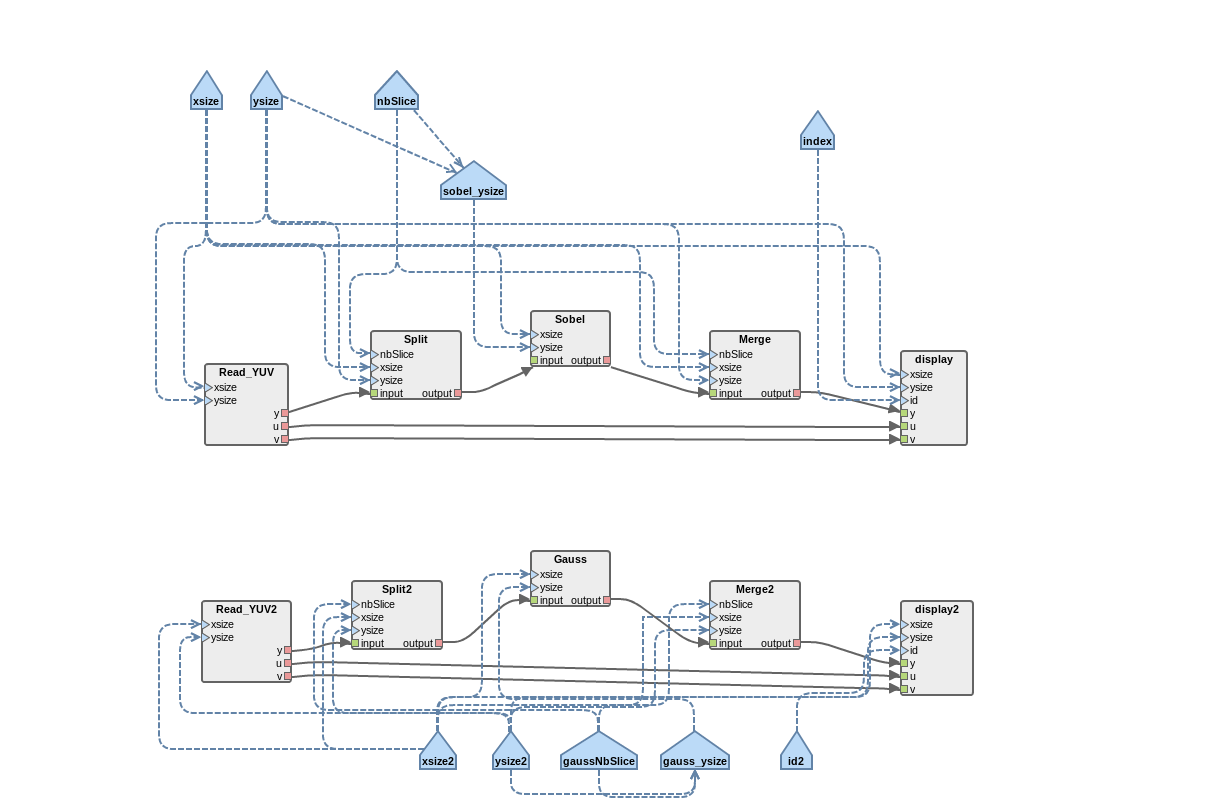
\includegraphics[width=0.99\textwidth]{images/preesm_diagram.png}
        \caption{The PiSDF graph of the PREESM filter application}
        \label{fig:preesm_actors}
    \end{center}
\end{figure}

\subsection{The Actor Model}
\label{subsec:actors}
To keep the model simple and the program well analyzable both of the processing paths in the network are independent. The first actor on both of the processing paths, the Read\_YUV and the Read\_YUV2 actors in the figure \ref{fig:preesm_actors}, loads the video frames from memory and passes them to splitting actors. The splitting actors split the frames to a suitable number of splices to enable processing of the same video stream on multiple cores. The filter actors, Sobel and Gauss actors in the figure, follow the splitting actors. Partial frames filtered in the filter actor are merged back to whole frames in the merge actors. The last actors on both of the processing paths are dummy actors. The pentagons in the top and the bottom of the figure represent the parameters of the application. The \texttt{xsize}, \texttt{ysize}, \texttt{xsize2} and \texttt{ysize2} parameters specify the size of the input frames. \texttt{nbSlice} and \texttt{gaussNbSlice} determine the numbers of slices the frames are split to. The \texttt{sobel\_ysize} and \texttt{gauss\_ysize} are the heights of the slices after splitting.

The first actors Read\_YUV and Read\_YUV2 call the \texttt{readYUV} function defined in the PREESM example at \cite{preesmtut}. As I/O is not in the scope of the experiments it is omitted from the application. The processing starts with loading the frames from memory. In a real world application the frames would be written to the memory for example with DMA by a packet processor processing a stream of network packets. The \texttt{readYUV} function copies the Y component of the input frame to the output address while the U and V components are ignored. The U and V are omitted because the sobel and gauss actors only operate on the Y channel in the experiment setup.

The split actor operates on the output of the Read\_YUV actor. The split actor preprocesses the frame for the sobel and gauss actors. Since the sobel and gauss filters involve convolution with 3x3 and 5x5 matrices respectively, they will need to access image data outside the part of the image they are processing. To enable parallel processing of a single frame on multiple cores, the frame is split in to slices. These slices will also need to contain a bit of extra data so that the filters can operate correctly. Black lines, or lines with the Y value of 0 are added to the top and the bottom of the frame. One black line is enough for the sobel frames but two black lines are needed for the gaussian frames, corresponding to the filter kernel sizes. After the padding, the slices overlap each other for one or two lines again corresponding to the size of the filter kernel. With the black lines added the frame is copied to the output buffer one slice at a time. 

The sobel actor calculates the convolution of the sobel kernels in presented in \ref{fig:sobelmat} with the Y component of the input frame. The sobel actor from from the PREESM example at \cite{preesmtut} is used in this experiment as well. The convolution is computed by looping over the pixels in the input frame, calculating the $G_{x}$ and $G_{y}$ components of the sobel operator and combining them by computing the average of absolute values of $G_{x}$ and $G_{y}$. After looping over the image the actor overwrites the edges of the frame with black pixels.

The gauss actor operates similarly to the sobel actor but instead of closed expressions the value of the filter function at each points is calculated by looping over the neighboring pixels and multiplying the intensity values by the corresponding weight from the gaussian kernel presented in \ref{fig:gaussmat}.

The last actor processing the frame is the merge actor. The merge actor copies the processed data from its input buffer to its output buffer, overlaying the slices so that the output frame doesn't contain the extra lines created in the split actor. Since there is no real I/O in the application, the merged frame is not processed further. In a real world application the processed frame would be copied for example to a network packet. As there is no I/O the display actors don't do any computations. In the experiments the display actor is used as the endpoint of the processing and it starts the data export.

\subsection{The PREESM Schedule}
\label{subsec:preesmsched}
The scheduler in the PREESM framework is described in \ref{sec:preesm-scheduling}. The scheduler creates a block schedule from the actor model using user provided estimates for the actor durations. To get reasonably accurate estimates, the application was first scheduled with the default values and the actor durations were measured on the target device. The resulting timings are presented in the table \ref{tab:preesm_times}. The timings from the measurements were approximately the same for all the actors except for the gauss actor. A gantt chart representing the schedule created using the values in the table is presented in figure \ref{fig:preesm_gantt}. The mutable parameters in the graph \ref{fig:preesm_actors} affect the static memory allocations of the PREESM application and the PREESM codegen workflow needs to be executed every time the parameters are changed. Because of this the PREESM schedules of the different measurement setups are slightly different.

\begin{table}
    \begin{center}
        \begin{tabular}{| c | c |}

            \hline
            Cycles & Actor \\ \hline
            600 & Gauss \\ \hline
            150 & Merge \\ \hline
            150 & Merge2 \\ \hline
            150 & Read\_YUV \\ \hline
            150 & Read\_YUV2 \\ \hline
            150 & Sobel \\ \hline
            150 & Split \\ \hline
            150 & Split2 \\ \hline
            1 & display \\ \hline
            1 & display2 \\ \hline
        \end{tabular}
        \caption{PREESM Actor Timings.}
        \label{tab:preesm_times}
    \end{center}
\end{table}

The PREESM framework doesn't support changing the timing of the implode and explode operations which started affecting the schedule considerably with larger frame sizes. The duration estimates used by PREESM for the implode and explode operations are very short compared to durations of the actors measured from the application. The explode operations for both streams are represented in the gantt chart by the small time slices predecing gauss actors on cores 4 and 7. The implode operation for gauss stream follows the gauss actor execution on core 7 and the implode operation of sobel stream follows the latter sobel actor on core 5.

\begin{figure}[h!]
    \begin{center}
        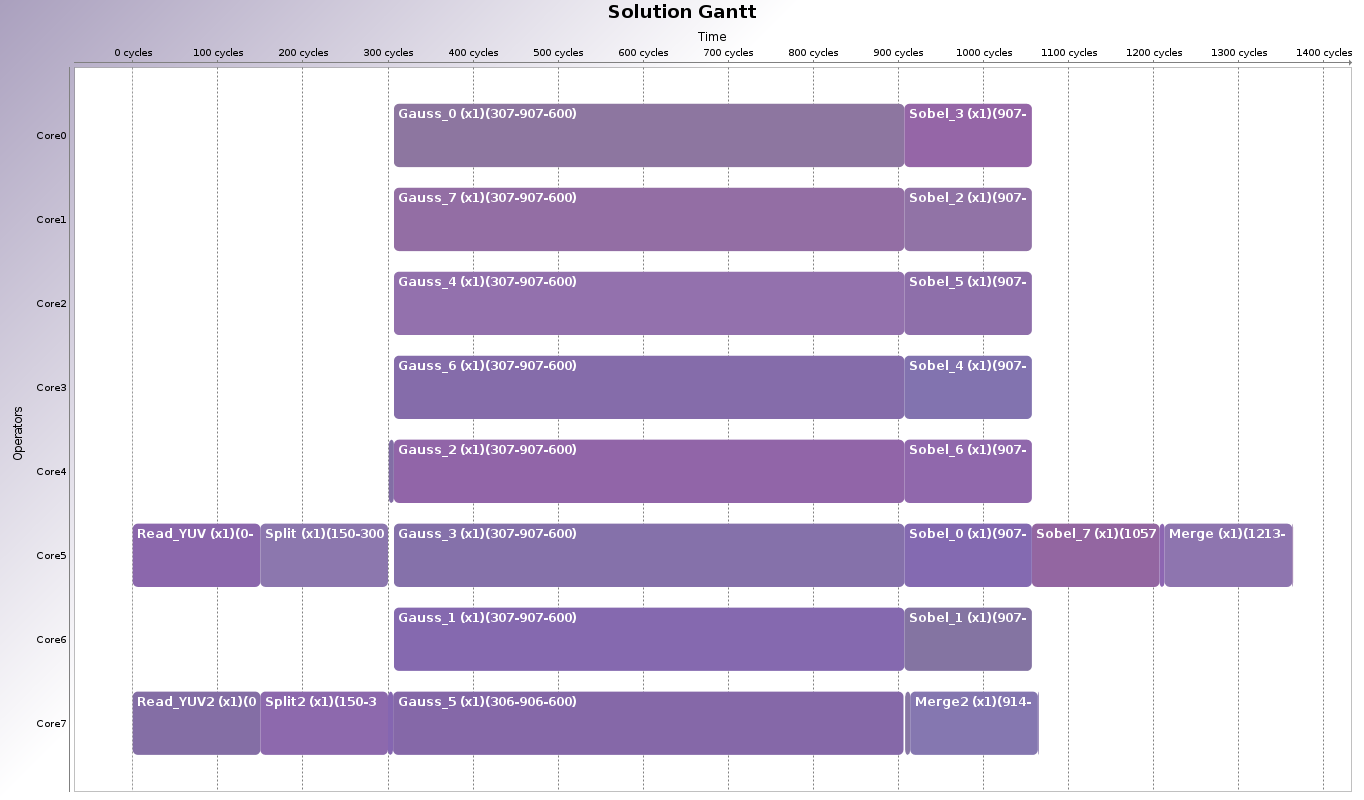
\includegraphics[width=0.99\textwidth]{images/gantt_preesm_cifcif.png}
        \caption{Gantt chart representing the schedule of a PREESM Filter Application.}
        \label{fig:preesm_gantt}
    \end{center}
\end{figure}

A block schedule could be generated, which would yield a higher throughput by introducing multiple instances of the actors for each repetition of the schedule. The successive repetitions of the schedule would be interleaved and the overhead of synchronizing the cores would be reduced. The current version of PREESM does not support the described interleaving of the repetitions \cite{pelcat2014preesm}.

\section{OpenEM Filter Application}
\label{sec:oemapp}
The OpenEM implementation of the filter application was designed using the PREESM filter application described in \ref{sec:preesmapp} as the starting point. Specifically the OpenEM application has to process the frames in similar manner so that only the scheduling policies between the two programming models should differ. The high-level structure of the OpenEM filter application is presented in the figure \ref{fig:openem_flow}. The application consists of two atomic queues, a parallel queue and three execution objects. Each queue is connected to only one execution object. The execution runs in cycles. A new cycle is started every time a cycle finishes. There are multiple cycles running in parallel, but since the read and merge EOs are atomic, only filter EO is running on multiple cores in parallel.

The design principles introduced in the beginning of this chapter apply to the OpenEM application as well. The OpenEM application was not designed for maximum performance but to demonstrate the suitability of OpenEM as a platform for stream processing applications. The performance of the application could be improved in many ways, for example by minimizing the amount of redundant copying of the frame slices and introducing parallelism to frame reading and merging.  

\begin{figure}[h!]
    \begin{center}
        \usetikzlibrary{chains}

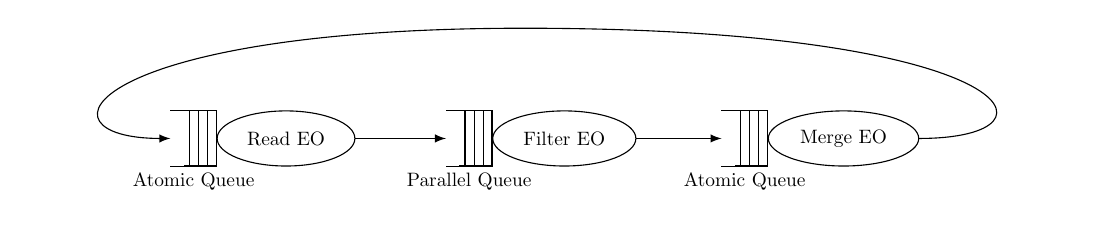
\begin{tikzpicture}[>=latex,node distance=0pt, scale=0.7, every node/.style={transform shape}]
    % the rectangular shape with vertical lines
    \node[rectangle split, rectangle split parts=6,
    draw, rectangle split horizontal,text height=0.5cm,text depth=0.5cm,inner sep=0pt, text width=0.0cm] (atomic1) {};
    \fill[white] ([xshift=-\pgflinewidth,yshift=-\pgflinewidth]atomic1.north west) rectangle ([xshift=-5pt,yshift=\pgflinewidth]atomic1.south);

    \node[draw,ellipse,right= 0pt of atomic1,minimum height=1.0cm,inner xsep=5pt] (readEO) {Read EO};

    \node at (5, 0)[rectangle split, rectangle split parts=6,
    draw, rectangle split horizontal,text height=0.5cm,text depth=0.5cm,inner sep=0pt, text width=0.0cm ] (parallel) {};
    \fill[white] ([xshift=-\pgflinewidth,yshift=-\pgflinewidth]parallel.north west) rectangle ([xshift=-5pt,yshift=\pgflinewidth]parallel.south);

    \node[draw,ellipse,right= 0pt of parallel,minimum height=1.0cm,inner xsep=5pt] (filterEO) {Filter EO};

    \node at (10, 0)[rectangle split, rectangle split parts=6,
    draw, rectangle split horizontal,text height=0.5cm,text depth=0.5cm,inner sep=0pt, text width=0.0cm] (atomic2) {};
    \fill[white] ([xshift=-\pgflinewidth,yshift=-\pgflinewidth]atomic2.north west) rectangle ([xshift=-5pt,yshift=\pgflinewidth]atomic2.south);

    \node[draw,ellipse,right= 0pt of atomic2,minimum height=1.0cm,inner xsep=5pt] (mergeEO) {Merge EO};

    % the arrows and labels
    \draw [->](readEO) to (parallel);
    \draw [->](filterEO) to (atomic2);
    \draw [->](mergeEO) .. controls (16,0) and (15, 2) .. (6, 2) .. controls (-2, 2) and (-3, 0) .. (atomic1);

    \node[align=center,below] at (atomic1.south) {Atomic Queue};
    \node[align=center,below] at (parallel.south) {Parallel Queue};
    \node[align=center,below] at (atomic2.south) {Atomic Queue};
\end{tikzpicture}

        \caption{The OpenEM filter application.}
        \label{fig:openem_flow}
    \end{center}
\end{figure}

The application execution starts with initializing the OpenEM framework and the application data structures. The OpenEM initialization is explained in \ref{subsec:ti-init-layer}. After the queues and the execution objects have been initialized the application creates a number of initial events that are sent to the the read queue. Once the events have been queued the application synchronizes all cores and the actual execution starts.

The Read EO combines the functionality of the read and split actors of the PREESM filter application presented in \ref{fig:preesm_actors}. A frame is read from the input video memory and split into a number of slices. The functions called are exactly the same as in the PREESM application. The frame slices are copied to event buffers of new events. The new events are then sent to the filter queue. There is only one filter queue and one filter execution object. The same execution object will compute either sobel or gauss filter on the frame slice according to its type.

The PREESM application splits the frames into slices and processes the slices separately before merging them back into one frame. Similar fork-join mechanism was implemented in the OpenEM application. Frames are accumulated simply in a merge buffer located in shared memory which is referenced through queue context pointers. The bookkeeping for frame completion is handled in the shared memory as well.

The filtered frame slices are accumulated in the merge buffer, which is accessed through the merge queue context. The merge queue is atomic to avoid need for synchronization between the cores. After a frame has been merged the merge EO creates a new event which is sent to the read queue. The ratio of sobel filtered frames to gauss filtered frames is always one to one.

\section{Instrumentation}
\label{sec:instrumentation}
To understand the behavior and performance of the applications their execution needs to be measured. The measurements conducted in the experiments were based on cycle counts. The TMS320C6678 exposes cycle counts on each core through two registers, namely TSCL and TSCH which store the low 32 bits and the high 32 bits of the cycle count respectively. Comparing the values of the TSCL register in the beginning and the end of processing on each core gives accurate local timings and would be enough for measuring the execution on single core. However for accurate measurements of global cycles, the cycle offsets to the global cycle count needed to be stored. The functionality for counting cycles was included in the Texas Instruments OpenEM initialization and utilities code. The cycle counts were stored in the DDR memory.

The latency of both of the filters is measured from the time the frame is loaded from the memory to the time the frame is merged after filtering. The throughput is measured as frames per second processed in total by the application. Since both of the applications process frames at the same rate from both streams, there is only one FPS measurement for each of the measurement setups.

In the PREESM application the cycle counts were saved in the beginning and the end of each user defined function of the application. In addition to this total cycle count was measured in the \texttt{readYUV} function. In the OpenEM application cycle counts were measured over the same functions as in the PREESM application and in the beginning and in the end of each EO. The latter measurements were carried out to get a better understanding of the OpenEM runtime overhead.

The measurements were exported through the debug connection of the TMS320C6678 using I/O library provided by Texas Instruments.

\section{Description of Experiments}
\label{sec:experiment-description}
In these experiments the OpenEM and PREESM filter applications were loaded with similar workloads and their execution was measured. The idea of the experiments is to examine the dynamic scheduling capabilities of the OpenEM scheduler and the overhead of the OpenEM framework in stream processing. The OpenEM scheduler is hardware accelerated, running on a separate processor in the TMS320C6678 chip. The scheduling is explained in detail in chapter \ref{chapter:openem}. To achieve this objective the OpenEM filter application introduced in chapter \ref{chapter:construction} was measured under different loads and compared to a similar application implemented using PREESM. The PREESM application should be considered a baseline, which demonstrates how a statically scheduled application behaves under dynamic workload.

The static schedule of the PREESM application was regenerated between every measurement setup due to the limitations of the code generation in PREESM framework. The specific limitation was that the parameters of the actor model were translated into static memory allocations in the code generator, and manually changing the generated allocations would have been complicated and prone to error. As a result the actors are scheduled slightly differently between each scenario. The schedules differ in the mapping of actors to cores but not in the ordering of the actors. The actor ordering is defined by the dependencies between the actors and availability of computing resources. The estimated actor timings of the PREESM application were not modified when changing the frame size.

In the experiments the applications are loaded with three different workloads and measured. In addition the OpenEM application is measured under the same load but different numbers of available cores. The experiments are described in the following subsections. In the first subsection the parameters and factors of the experiment are introduced. Second the different measurement setups are described and third the results of the experiment are presented.

\subsection{Parameters and Factors}
\label{subsec:parameters-and-factors}
Dynamic workload conditions are emulated by repeating the measurements with different factors. To keep the measurement setup simple the video streams are not dynamically switched at runtime. The measurement parameters are presented in the following listing.

\begin{itemize}
    \item \textbf{Video Frame Size} - The workloads are differentiated by changing the frame sizes of the video streams.
    \item \textbf{OpenEM Core Masks} - The OpenEM application is measured with different core masks of the Execution Objects.
    \item \textbf{Number of Frames Processed Simultaneously} - The OpenEM application processes variable number of frames simultaneously.
\end{itemize}

The different video frame sizes used are presented in table \ref{tab:cif_frames}. The frame sizes used are selected from among the Common Intermediate Format frame sizes. YUV video format is used in the applications, but only the Y channel is processed by the applications. The Y channel in the YUV frame contains $R_{x} * R_{y}$ bytes where $R$ is the resolution. In the YUV format used the U and V channels have reduced bitrates of $\frac{1}{4} * R_{x} * R_{y}$ per frame.

\begin{table}
    \begin{center}
        \begin{tabular}{ c c c }
            Name  & X resolution  & Y resolution \\ \hline
            QCIF  & 176           & 144          \\ \hline
            CIF   & 352           & 288          \\ \hline
            4CIF  & 704           & 576          \\ \hline
        \end{tabular}
        \caption{CIF frame sizes}
        \label{tab:cif_frames}
    \end{center}
\end{table}

The OpenEM application circulates the events created initially throughout its lifetime. The number of initial events determines the maximum number of frames that can be processed simultaneously. The effect of the number of the simultaneously processed frames to the latency and throughput of the application is examined in the experiments.

OpenEM core masks are used to limit the number of cores available to the filter application. The behavior of OpenEM is examined under limited resources. With the use of core masks the performance improvement through increased parallelism is investigated.

\subsection{Measurement Setups}
\label{subsec:measurement-setups}
The filter applications process two video streams simultaneously as described in chapter \ref{chapter:construction}. One video stream is processed with a sobel filter and the other is processed with a gaussian filter. The dynamic behavior of the applications is investigated using different workloads.

\begin{table}
    \begin{center}
        \begin{tabular}{ c c }
            Sobel Resolution & Gauss Resolution \\ \hline
            CIF              & CIF              \\ \hline
            4CIF             & CIF              \\ \hline
            CIF              & 4CIF             \\ \hline
            QCIF             & QCIF             \\ \hline
        \end{tabular}
        \caption{PREESM and OpenEM measurement setups}
        \label{tab:preesm_setups}
    \end{center}
\end{table}

\begin{itemize}
    \item \textit{Comparing Dynamic and Static Scheduling}
    The workloads used in the first experiment are presented in the table \ref{tab:preesm_setups}. The purpose of the different bitrates used for each video stream is to expose the behavior of the OpenEM scheduler in handling dynamic workloads. The static schedule in the PREESM application will provide a baseline to reflect the OpenEM performance to, but the performance of the applications should not be directly compared due to the difference in the runtime systems.

\item \textit{Investigating the Balance of Latency and Throughput}
To examine the capabilities of the dynamic scheduler the number of simultaneously processed events is varied in the second experiment. The maximum number of frames that can be processed simultaneously corresponds to the number of initial events created in the initialization. Both filters are loaded with CIF streams and the measurements are run with 1 to 24 initial events. The number of simultaneous frames changes the throughput versus latency balance of the OpenEM application.

\item \textit{Examining the Efficiency of Parallel Scheduling}
In the third experiment the OpenEM application is measured with different core masks to investigate the ability of the dynamic scheduler to utilize the increased parallel resources. Both filters of the OpenEM application are loaded with CIF streams. Different numbers of cores are used, but all actors can run on all available cores. The experiment is run with core masks allowing one to eight cores be used for processing the streams. The experiment is run with 16 initial events.
\end{itemize}

\chapter{Experiment Results and Analysis}
\label{chapter:results-and-analysis}
The results of the experiments conducted in this thesis are presented in this chapter. The section \ref{sec:results} presents and describes the results. A more in-depth look at the results is taken in \ref{sec:discussion} where the results are discussed and their significance assessed.

\section{Results}
\label{sec:results}
In this section the results of the three experiments described in~\ref{subsec:measurement-setups} are described. The results of the comparison of the application using the OpenEM dynamic scheduler and the statically scheduled application created with PREESM is given in~\ref{subsec:first-experiment}. The results of the experiment investigating the balance of latency versus throughput are given in~\ref{subsec:second-experiment}. Finally, the results of the third experiment examining the efficiency of increasing the parallelism in the dynamically scheduled application are given in~\ref{subsec:third-experiment}.

\subsection{Comparing Dynamic and Static Scheduling}
\label{subsec:first-experiment}
\FloatBarrier
In the first experiment the bitrates of the two video streams are varied. The latency and throughput of the OpenEM application measurements are summarized in the table \ref{tab:oemthrough2}. The corresponding summaries for the PREESM application are presented in the table \ref{tab:preesmthrough} 

The latencies of the two streams of the PREESM application in all measurement setups in the table \ref{tab:preesmthrough} are similar. The largest difference in the latencies is in the case where sobel filter filters a CIF stream and gauss filter filters a 4CIF stream, where gauss latency is 60\% higher than the sobel latency. Much larger differences in the latencies are observed with the OpenEM application with two initial events presented in table \ref{tab:oemthrough2} where the largest difference in latencies is also measured between the CIF sobel stream and 4CIF gauss stream. The gauss latency in the particular OpenEM measurement is 200\% higher than the sobel latency. The other OpenEM measurements show larger differences as well compared to PREESM.

\newcommand{\head}[2]{\multicolumn{1}{>{\centering\arraybackslash}p{#1}}{#2}}
\begin{table}
    \begin{center}
        \begin{tabular}{ c c c c c }
            \head{1.5cm}{Sobel latency} & \head{1.5cm}{Gauss latency} &
            \head{1.5cm}{FPS} & \head{1.5cm}{Sobel frame} &
            \head{1.5cm}{Gauss frame} \\ \hline
            5,41 & 8,78 & 223 & CIF & 4CIF \\ \hline
            4,65 & 3,54 & 334 & 4CIF & CIF \\ \hline
            2,15 & 2,51 & 668 & CIF & CIF \\ \hline
            0,61 & 0,71 & 2004 & QCIF & QCIF \\ \hline
        \end{tabular}
        \caption{PREESM latency and throughput. The the latencies are measured in milliseconds.}
        \label{tab:preesmthrough}
    \end{center}
\end{table}
\begin{table}
    \begin{center}
        \begin{tabular}{ c c c c c }
            \head{1.5cm}{Sobel latency} & \head{1.5cm}{Gauss latency} &
            \head{1.5cm}{FPS} & \head{1.5cm}{Sobel frame} &
            \head{1.5cm}{Gauss frame} \\ \hline
            3,59 & 10,93 & 256 & CIF & 4CIF \\ \hline
            3,75 & 2,95 & 527 & 4CIF & CIF \\ \hline
            1,42 & 2,80 & 889 & CIF & CIF \\ \hline
            0,32 & 0,71 & 3534 & QCIF & QCIF \\ \hline
        \end{tabular}
        \caption{OpenEM latency and throughput with 2 frames processed simultaneously. The latencies are measured in milliseconds.}
        \label{tab:oemthrough2}
    \end{center}
\end{table}

The throughput of the application is determined by how much time the application spends processing the streams versus the time spent doing something else. For example the synchronization of all cores before each repetition of the PREESM schedule consumes a lot of CPU cycles as is readily observed from the figure \ref{fig:preesmcif}. The portion of the bars marked as busy corresponds to the cycles spent in the synchronization between the repetitions of the schedule. The percentage of cycles spent in the synchronization varies from 16\% on Core 7 to 45\% on Core 0. The OpenEM dynamic scheduler seems to spread out the work more evenly in this case where the total overhead cycles are approximately 60\% for all cores. The core utilization per function is presented in figure \ref{fig:oem8corefunc}. Most of the overhead cycles in the OpenEM application are spent waiting for more frames for processing.

\begin{figure}
    \centering
    \begin{subfigure}[t]{0.49\textwidth}
        \centering
        \includegraphics[width=0.99\linewidth]{images/preesm_cifcif.eps}
        \caption{PREESM}
        \label{fig:preesmcif}
    \end{subfigure}
    \begin{subfigure}[t]{0.49\textwidth}
        \centering
        \includegraphics[width=0.99\linewidth]{images/openem_cifcif_2initial_func.eps}
        \caption{OpenEM}
        \label{fig:oem8corefunc}
    \end{subfigure}
    \caption{In the PREESM graph the busy portion of the bars correspond to the cycles spent synchronizing the cores between the repetitions of the block schedule. The overhead corresponds to cycles spent outside the measured functions and the synchronization. In the OpenEM application the overhead cycles are the cycles spent outside the compared functions.}
\end{figure}

The overhead portions in the figures \ref{fig:preesmcif} and \ref{fig:oem8corefunc} contain all of the data copying from buffer to buffer outside the measured functions, but they also contain different amounts of cycles spent in communications between the cores. The measured functions are the functions which are explicitly called in the PREESM actor model. Other functions not included in the measured functions contain runtime specific communication and some copying of buffers.

\FloatBarrier
\subsection[Investigating the Balance of Latency and Throughput]{Investigating the Balance of Latency\\and Throughput}
\label{subsec:second-experiment}
\FloatBarrier
\begin{table}
    \begin{center}
        \begin{tabular}{ c c c c c }
            \head{1.5cm}{Sobel latency} & \head{1.5cm}{Gauss latency} &
            \head{1.5cm}{FPS} & \head{1.5cm}{Sobel frame} &
            \head{1.5cm}{Gauss frame} \\ \hline
            15,82 & 22,85 & 599 & CIF & 4CIF \\ \hline
            4,85 & 3,67 & 895 & 4CIF & CIF \\ \hline
            4,91 & 5,96 & 1955 & CIF & CIF \\ \hline
            1,33 & 1,62 & 7819 & QCIF & QCIF \\ \hline
        \end{tabular}
        \caption{OpenEM latency and throughput with 16 frames processed simultaneously. The latencies are measured in milliseconds.}
        \label{tab:oemthrough}
    \end{center}
\end{table}
The PREESM latencies in the table \ref{tab:preesmthrough} are consistently smaller than the latencies of the throughput optimized OpenEM application in the table \ref{tab:oemthrough}. In this set of measurements the OpenEM application is configured to process 16 frames simultaneously to maximize throughput. The throughput of the OpenEM application is almost doubled compared to the configuration presented in \ref{tab:oemthrough2} where two frames processed simultaneously.

The effect of increasing the number of simultaneous frames was further examined by measuring the application with two CIF streams using 2 to 24 initial events. The results of the measurements are presented in table \ref{tab:oeminitialframes}. The latencies get worse and the throughput gets better when the number of frames processed simultaneously increases. This behavior is visualized in figures \ref{fig:oeminitialframesfps} and \ref{fig:oeminitialframeslat}. The throughput grows rapidly up to 8 simultaneous frames after which the growth slows down. The latencies grow with each added frame steadily.
\begin{figure}
    \centering
    \begin{subfigure}[t]{0.49\textwidth}
        \centering
        \includegraphics[width=0.99\linewidth]{images/simultaneous_frames_fps.eps}
        \caption{FPS as a function of simultaneous frames.}
        \label{fig:oeminitialframesfps}
    \end{subfigure}
    \begin{subfigure}[t]{0.49\textwidth}
        \centering
        \includegraphics[width=0.99\linewidth]{images/simultaneous_frames_latency.eps}
        \caption{Latencies as functions of simultaneous frames. The latencies are measured in milliseconds.}
        \label{fig:oeminitialframeslat}
    \end{subfigure}
    \caption{The effect of increasing the number of frames processed simultaneously is presented in the figures. The throughput increases rapidly up to 8 simultaneous frames after which the growth slows down. The latency grows more steadily across all measured setups.}
\end{figure}
\begin{table}
    \begin{center}
        \begin{tabular}{ c c c c }
            \head{1.5cm}{Sobel latency} & \head{1.5cm}{Gauss latency} &
            \head{1.5cm}{FPS} & \head{1.5cm}{Simultaneous Frames} \\
            \hline
            1,42  &  2,80  &  889   &  2 \\ \hline
            1,72  &  3,22  &  1371  &  4 \\ \hline
            2,26  &  3,59  &  1655  &  6 \\ \hline
            2,67  &  3,96  &  1825  &  8 \\ \hline
            3,13  &  4,37  &  1880  &  10 \\ \hline
            3,68  &  4,89  &  1921  &  12 \\ \hline
            4,27  &  5,40  &  1940  &  14 \\ \hline
            4,73  &  5,88  &  1958  &  16 \\ \hline
            5,43  &  6,52  &  1976  &  18 \\ \hline
            6,22  &  7,21  &  1983  &  20 \\ \hline
            6,83  &  7,80  &  1981  &  22 \\ \hline
            7,41  &  8,45  &  1992  &  24 \\ \hline
        \end{tabular}
        \caption{OpenEM measurements with different numbers of frames in processed simultaneously.}
        \label{tab:oeminitialframes}
    \end{center}
\end{table}

\FloatBarrier
\subsection{Examining the Efficiency of Parallel Scheduling}
\label{subsec:third-experiment}
\FloatBarrier
\begin{table}
    \begin{center}
        \begin{tabular}{ c c c c }
            \head{1.5cm}{Sobel latency} & \head{1.5cm}{Gauss latency} &
            \head{1.5cm}{FPS} & \head{1.5cm}{Number of cores} \\
            \hline
            57,05 & 57,11 & 263 & 1 \\ \hline
            22,59 & 23,15 & 510 & 2 \\ \hline
            15,09 & 15,84 & 768 & 3 \\ \hline
            10,91 & 11,85 & 1014 & 4 \\ \hline
            8,41 & 9,53 & 1268 & 5 \\ \hline
            7,05 & 8,07 & 1500 & 6 \\ \hline
            5,74 & 6,83 & 1731 & 7 \\ \hline
            4,91 & 5,96 & 1955 & 8 \\ \hline
        \end{tabular}
        \caption{OpenEM measurements with number of cores varied}
        \label{tab:oemcoremasks}
    \end{center}
\end{table}

In the third experiment the number of cores available for the OpenEM application was varied. Both filters were processing CIF streams. The measurements were repeated using one to eight cores. The resulting latencies and throughputs are presented in the table \ref{tab:oemcoremasks}. The increase of the throughput of the OpenEM application is presented in graph \ref{fig:fpsvcores}. The actual FPS measured with eight cores is approximately 90\% of the linear growth calculated from the FPS using a single core.
\begin{figure}
    \begin{center}
        \includegraphics[width=0.7\textwidth]{images/coremask_fps.eps}
        \caption{FPS increase as the function of cores vs. linear growth}
        \label{fig:fpsvcores}
    \end{center}
\end{figure}
\FloatBarrier

\section{Discussion}
\label{sec:discussion}
Three experiments were conducted to understand the performance of OpenEM in stream processing. Stream processing application was implemented with OpenEM and a comparable application was implemented using PREESM. The performance of the application as a part of a stream processing system was not studied. Therefore IO was omitted from the stream processing task that both of the applications implemented.  The experiments focused on understanding the performance of the OpenEM scheduler in handling stream processing tasks.

In this section the results of the three conducted experiments are discussed. First the discoveries made from the experiments are described in \ref{subsec:discoveries}. Second the possible directions of future work are discussed in \ref{subsec:future-work}. Finally the challenges faced conducting the experiments are explained in \ref{subsec:challenges}

\subsection{Discoveries}
\label{subsec:discoveries}
\FloatBarrier
The first experiment where the throughput and latency of OpenEM were compared to those of PREESM showed that the runtime systems are roughly comparable. The statically scheduled application created with PREESM potentially had the advantage here, since with static schedule no cycles are wasted at any point in the execution in deciding which actor to execute next on which core. OpenEM achieved very similar latencies with the dynamic scheduler. This suggests that the OpenEM scheduler utilizes the hardware resources efficiently and causes relatively small overhead.

The PREESM authors state that PREESM is a prototyping tool~\cite{preesm}, which suggests that it does not necessarily aim to create latency or throughput optimized applications. The Gantt chart in figure~\ref{fig:preesm_gantt} suggests that manually optimizing the schedule, a lower latency and higher throughput could be achievable. This is supported by the core utilization graph in figure~\ref{fig:preesmcif} where a large portion of the execution time is spent waiting for other cores. Nevertheless, the OpenEM scheduling performance can be considered good as it roughly matches the statically generated schedule.

In the second experiment the balance of latency versus throughput with the OpenEM scheduler was investigated. The experiment where the number of simultaneously processed frames was varied suggested that by configuring the application the balance between throughput and latency can be controlled. The adjustability of the scheduler is a useful feature to have in real applications, as the throughput can be increased for tasks, which are less latency sensitive without modifying the program code. The extent of control the application designer has depends on the complexity of the application. The application measured in the experiments was simple and it is possible that the results overemphasize the adaptivity compared to more complex applications.

The third experiment was conducted to understand the performance improvement gained from making more processing units available for the runtime. The FPS improvement from one to eight cores is close to 90\% of linear improvement. This means that the sequential portion of the application was small and the scheduler was able to utilize the increased parallelism efficiently.

Since two frames are processed simultaneously the execution of the serial part of the program performed in the read and merge execution objects is interleaved with the execution of the filter execution object of the other frame. This behavior seems to yield a large latency decrease from execution on one core to execution on two cores. Unfortunately this complicates the analysis, since the proportion of the serial and parallel parts of the program is ambiguous. This complication prevents useful comparisons with the theoretical improvement defined by Amdahl's law~\cite{amdahl1967validity}.

The result of the parallel scheduling experiment was not surprising but it is reassuring of the OpenEM scheduler performance. As the total number of events in circulation was quite small compared to the example applications, the scheduler should have no trouble keeping up with the pace of the application even with eight cores.

\begin{figure}
    \centering
    \begin{subfigure}[t]{0.49\textwidth}
        \centering
        \includegraphics[width=0.99\linewidth]{images/openem_cifcif_8cores_eo.eps}
        \caption{Sobel CIF, Gauss CIF}
        \label{fig:oem8coreeo}
    \end{subfigure}
    \begin{subfigure}[t]{0.49\textwidth}
        \centering
        \includegraphics[width=0.99\linewidth]{images/openem_sobel4cif_gausscif_eo.eps}
        \caption{Sobel 4CIF, Gauss Cif}
        \label{fig:oem8coreeosobel4cif}
    \end{subfigure}
    \caption{The bottleneck forming due to the atomic read operation can be observed by comparing the core utilization when both of the streams are at CIF resolution to the case where sobel resolution is increased to 4CIF. In these graphs the application is processing 16 simultaneous events.}
\end{figure}

The throughput optimized application processing 16 events simultaneously exhibits formation of a bottleneck in the atomic execution object. In the table \ref{tab:oemthrough} an improvement of latencies is observed when the workload is made heavier by moving 4CIF stream from gauss filter to the sobel filter while the other stream is kept at CIF resolution.

The probable cause of the improvement of the latencies when the workload is made heavier by increasing the sobel stream resolution is the reduced interleaving of the processing of the subsequent frames. The reduction in the interleaving is caused by the read execution object which is only connected to an atomic queue. When the frame size of the sobel stream is increased the read EO starts limiting the throughput of the application. Fewer frames are processed in parallel which decreases the time from reading each individual frame to the completion of that frame.

The formation of the bottleneck can be observed by comparing the core utilization in the figure \ref{fig:oem8coreeo} to the core utilization in the figure \ref{fig:oem8coreeosobel4cif} where seven cores need to wait for the read operations on the Core 2 and the overall overhead is increased. The other cores do not receive any events from the OpenEM scheduler while waiting.

\begin{figure}[h]
    \begin{center}
        \includegraphics[width=0.49\textwidth]{images/openem_sobelcif_gauss4cif_eo.eps}
        \caption{OpenEM cycles spent per execution object for CIF sobel frames
        and 4CIF gauss frames}
        \label{fig:oem8coreeogauss4cif}
    \end{center}
\end{figure}

When the gauss stream is increased to 4CIF and the sobel stream is kept at CIF the bottleneck does not form. This is likely because computing the gaussian filter for the 4CIF frames is consuming approximately 80\% of the cycles on all cores. In this case the read EO only consumes approximately 5\% to 13\% of the cycles on all cores. Compared to the case of two CIF streams, the latencies in this case are increased by factors of approximately 3 and 4 for sobel and gauss correspondingly. The resulting core utilization graph is presented in figure \ref{fig:oem8coreeogauss4cif}.
\FloatBarrier

\subsection{Future Work}
\label{subsec:future-work}
In this thesis the use of OpenEM to provide task management and scheduling in a stream processing application was investigated. The results suggest that OpenEM scales well to the needs of a simple stream processing application and it simplifies the implementation of a multi-core application on the DSP platform without operating system.

The workload studied in this thesis was simple and lacked dynamicity of processing graphs common to stream processing applications. To better understand the performance of OpenEM, two future research approaches could be taken. First, studying the performance of OpenEM scheduler with another artificial workload application could still strengthen the case for using OpenEM as the runtime for stream processing. Instead of a simple, linear processing graph like the one used in the experiments of this thesis, a more dynamic graph with optional processing paths could be studied. Studying this kind of graph would show if the scheduler is capable of hitting the latency and throughput constraints of the application consistently under varying load. Second, a more complex application could be constructed and measured. For example implementing an MPEG decoder using OpenEM as the runtime system would provide a more complete view to the dynamic performance of OpenEM. An MPEG decoder would be an interesting workload because it has been used as something of a standard benchmark in dataflow literature and thus there exists many implementations based on different technologies. Having points of comparison for the workload would help put the performance in broader context.

The idea of using DSPs for stream processing has been researched to some extent but the idea has not made it to the mainstream of computing industry. To make the case for DSPs as stream processors a thorough benchmark should be created that would compare the streaming performance versus energy consumed for similar stream processing applications implemented with DSPs, GPUs and CPUs. Making such comparison is not trivial, since to the author's knowledge there does not exist a single widely accepted measure of streaming performance. The question is complicated further by the need for measuring the energy consumption, which itself is a complex task.

Before conducting such research three problems would have to be solved. First, selection of the measured variables. Comparing floating point operations per second per Joule between the platforms would be the simple solution, but FLOPS is not necessarily good measurement for streaming performance. For example, for video stream frames per second and latency would provide a better understanding of the streaming performance than FLOPS. Second, accounting of the energy consumption fairly with all measured processing units is not trivial, since they are commonly installed in different forms of devices. CPUs are installed in sockets on motherboards, GPUs are installed on PCI cards or increasingly as part of integrated chips and DSPs are installed in various devices including PCI cards. Comparing the vendor provided energy specifications is one way to deal with this problem, but it might miss how the devices are actually deployed. Third, the workload would have to be implemented in different patterns for each of the platforms making use of the strengths of each platform equally.

Two papers conduct comparisons that partially answer the questions above, but do not actually provide the complete comparison between the processors. Stotzer et al. conduct an experiment in~\cite{stotzer2013openmp} where a comparison between the different processing units is conducted in the context of OpenMP, but the comparison does not include energy measurements. The performance of FPGAs and GPUs in processing what the author calls ``sliding-window applications'' is compared in terms of Joules per frame in~\cite{fowers2012performance}. The ``sliding-window applications'' consist of applying convolutions on frames of data in the stream, similar to how the workload in this thesis computes.

\subsection{Challenges}
\label{subsec:challenges}
Analysing the performance of OpenEM based stream processing applications is a broad task, requiring the use of many distinct technologies. First a suitable workload, which is representative of stream processing tasks had to be designed. Next two versions of the workload application had to be implemented, one for the evaluation of OpenEM and the other to provide a point of comparison. In order to get usable data from the applications, they had to be instrumented and the measurement data analysed. Most of the work required was straightforward but some complications were faced with the tools.

The baseline application was implemented using PREESM. PREESM generates static schedules for the application from provided the dataflow graph and the source code. To get specific points of comparison for each of the measurement setups working with the PREESM automatic code generation was complicated. The tool would create different schedules on each iteration and thus yield applications with dissimilar core usage between the measurement setups.

Texas Instruments OpenEM version 1.0.0.2 that was used for the implementation of the OpenEM workload has some unimplemented features. Most of the unimplemented features were documented and did not cause unnecessary work. However the implementation of Queue Groups did not work as expected. Creation of multiple queue groups did not work as specified in the documentation, and was left unexplored after multiple trials at working with them.

The documentation of the Texas Instruments implementation of OpenEM was lacking. The documentation provided with the source code was incomplete and included a sketchy version of the OpenEM white paper~\cite{moerman2014open} which was the most important source for understanding the use of hardware acceleration in the runtime. The documentation also lacked details for the initialization layer without which the initialization of the hardware components would have been difficult. The initialization code was provided as a part of a scarcely documented example application.

\chapter{Conclusions}
\label{chapter:conclusion}
This thesis set out to investigate the performance of OpenEM based stream processing applications, with specific focus on scheduling. Scheduling is an important factor of the streaming performance. A good scheduler is capable of utilizing parallelism to improve throughput and latency of the application, whereas worse schedulers do not distribute work on multiple cores as efficiently and thus execute more of the work sequentially leading to increased latency and decreased throughput.

The problem was approached by comparing the performance of an Open Event Machine based streaming application to the performance of a similar, statically scheduled application. The workload application designed for the experiments is a video stream processing application inspired by the Canny edge detector. The baseline application was implemented using PREESM, which generates statically scheduled multi-core applications based on synchronous dataflow graphs. The applications were instrumented so that they could be compared in terms of latency, throughput, and core utilization. The results of the comparison experiment suggest that the OpenEM dynamic scheduler does not cause unmanageable overhead compared to statically scheduled applications.

The scheduling performance of OpenEM was further investigated with two experiments carried out using the same measurement system. In one experiment the balance between throughput and latency was examined by increasing the number of frames processed concurrently. This experiment showed that at least simple OpenEM applications are adjustable in terms of throughput and latency, which may be useful in stream processing tasks. In the other experiment the parallelizing performance of the scheduler was examined by computing the same tasks using variable number of cores. The growth in performance was 90\% of linear growth from one to eight cores, which is decent improvement considering that in addition to the parallel actors, the workload had sequential actors, which did not benefit from the parallelization.

The results of the experiments suggest that Texas Instruments OpenEM runtime is flexible enough to support the implementation of streaming applications and it was found that the dynamic scheduler is capable of making reasonable scheduling decisions with small overhead. Further research is required to understand the overall performance of multi-core DSPs versus GPUs, FPGAs, and CPUs in stream processing.

As data streaming is becoming more widespread in the Internet, high performance stream processing solutions are in demand in the industry. Exploring the use of DSPs for stream processing is interesting because they achieve high ratio of floating point operations to energy consumption and they implement an architecture that is well suited to stream processing in theory. As multi-core DSPs are not as commonly used for stream processing as for example GPUs, the toolset for parallel programming is not as standardized as on other platforms. Therefore, runtime systems such as OpenEM have the potential of becoming the standard tools for stream processing on DSPs.

% Load the bibliographic references
% ------------------------------------------------------------------
% You can use several .bib files:
% \bibliography{thesis_sources,ietf_sources}
\bibliography{sources}


% Appendices go here
% ------------------------------------------------------------------
% If you do not have appendices, comment out the following lines
%\appendix
%\chapter{First appendix: OpenEM and PREESM comparison}
\label{chapter:first-appendix}

\begin{figure}[h!]
    \begin{center}
        \includegraphics[width=0.99\textwidth]{images/openem_cifcif_8cores_eo.eps}
        \caption{OpenEM cycles spent per execution object for CIF sobel frames and CIF gauss frames}
%        \label{fig:oem8coreeo}
    \end{center}
\end{figure}

\begin{figure}[h!]
    \begin{center}
        \includegraphics[width=0.99\textwidth]{images/openem_cifcif_8cores_func.eps}
        \caption{OpenEM cycles spent per function for CIF sobel frames and CIF gauss frames}
%        \label{fig:oem8corefunc}
    \end{center}
\end{figure}

\begin{figure}[h!]
    \begin{center}
        \includegraphics[width=0.99\textwidth]{images/openem_sobel4cif_gausscif_eo.eps}
        \caption{OpenEM cycles spent per execution object for 4CIF sobel frames and CIF gauss frames}
%        \label{fig:oem8coreeosobel4cif}
    \end{center}
\end{figure}

\begin{figure}[h!]
    \begin{center}
        \includegraphics[width=0.99\textwidth]{images/openem_sobel4cif_gausscif_func.eps}
        \caption{OpenEM cycles spent per function for 4CIF sobel frames and CIF gauss frames}
        \label{fig:oem8corefuncsobel4cif}
    \end{center}
\end{figure}

\begin{figure}[h!]
    \begin{center}
        \includegraphics[width=0.99\textwidth]{images/openem_sobelcif_gauss4cif_eo.eps}
        \caption{OpenEM cycles spent per execution object for CIF sobel frames and 4CIF gauss frames}
%        \label{fig:oem8coreeogauss4cif}
    \end{center}
\end{figure}

\begin{figure}[h!]
    \begin{center}
        \includegraphics[width=0.99\textwidth]{images/openem_sobelcif_gauss4cif_func.eps}
        \caption{OpenEM cycles spent per function for CIF sobel frames and 4CIF gauss frames}
        \label{fig:oem8corefuncgauss4cif}
    \end{center}
\end{figure}

\begin{figure}[h!]
    \begin{center}
        \includegraphics[width=0.99\textwidth]{images/openem_sobelqcif_gaussqcif_eo.eps}
        \caption{OpenEM cycles spent per execution object for QCIF sobel frames and QCIF gauss frames}
        \label{fig:oem8coreeoqcif}
    \end{center}
\end{figure}

\begin{figure}[h!]
    \begin{center}
        \includegraphics[width=0.99\textwidth]{images/openem_sobelqcif_gaussqcif_func.eps}
        \caption{OpenEM cycles spent per function for CIF sobel frames and 4CIF gauss frames}
        \label{fig:oem8corefuncqcif}
    \end{center}
\end{figure}

\begin{figure}[h!]
    \begin{center}
        \includegraphics[width=0.99\textwidth]{images/preesm_cifcif.eps}
        \caption{PREESM cycles spent per function for CIF sobel frames and CIF gauss frames}
%        \label{fig:preesmcif}
    \end{center}
\end{figure}

\begin{figure}[h!]
    \begin{center}
        \includegraphics[width=0.99\textwidth]{images/preesm_sobel4cif_gausscif.eps}
        \caption{PREESM cycles spent per function for 4CIF sobel frames and CIF gauss frames}
        \label{fig:preesmsobel4cif}
    \end{center}
\end{figure}

\begin{figure}[h!]
    \begin{center}
        \includegraphics[width=0.99\textwidth]{images/preesm_sobelcif_gauss4cif.eps}
        \caption{PREESM cycles spent per function for CIF sobel frames and 4CIF gauss frames}
        \label{fig:preesmgauss4cif}
    \end{center}
\end{figure}

\begin{figure}[h!]
    \begin{center}
        \includegraphics[width=0.99\textwidth]{images/preesm_sobelqcif_gaussqcif.eps}
        \caption{PREESM cycles spent per function for QCIF sobel frames and QCIF gauss frames}
        \label{fig:preesmgauss4cif}
    \end{center}
\end{figure}


\chapter{Second Appendix: OpenEM coremasks}

\begin{figure}[h!]
    \begin{center}
        \includegraphics[width=0.99\textwidth]{images/openem_cifcif_1cores_eo.eps}
        \caption{OpenEM cycles spent per execution object for CIF sobel frames and CIF gauss frames using 1 core.}
        \label{fig:oem1coreeo}
    \end{center}
\end{figure}

\begin{figure}[h!]
    \begin{center}
        \includegraphics[width=0.99\textwidth]{images/openem_cifcif_1cores_func.eps}
        \caption{OpenEM cycles spent per function for CIF sobel frames and CIF gauss frames using 1 core.}
        \label{fig:oem1corefunc}
    \end{center}
\end{figure}


\begin{figure}[h!]
    \begin{center}
        \includegraphics[width=0.99\textwidth]{images/openem_cifcif_2cores_eo.eps}
        \caption{OpenEM cycles spent per execution object for CIF sobel frames and CIF gauss frames using 2 cores.}
        \label{fig:oem2coreeo}
    \end{center}
\end{figure}

\begin{figure}[h!]
    \begin{center}
        \includegraphics[width=0.99\textwidth]{images/openem_cifcif_2cores_func.eps}
        \caption{OpenEM cycles spent per function for CIF sobel frames and CIF gauss frames using 2 cores.}
        \label{fig:oem2corefunc}
    \end{center}
\end{figure}


\begin{figure}[h!]
    \begin{center}
        \includegraphics[width=0.99\textwidth]{images/openem_cifcif_3cores_eo.eps}
        \caption{OpenEM cycles spent per execution object for CIF sobel frames and CIF gauss frames using 3 cores.}
        \label{fig:oem3coreeo}
    \end{center}
\end{figure}

\begin{figure}[h!]
    \begin{center}
        \includegraphics[width=0.99\textwidth]{images/openem_cifcif_3cores_func.eps}
        \caption{OpenEM cycles spent per function for CIF sobel frames and CIF gauss frames using 3 cores.}
        \label{fig:oem3corefunc}
    \end{center}
\end{figure}


\begin{figure}[h!]
    \begin{center}
        \includegraphics[width=0.99\textwidth]{images/openem_cifcif_4cores_eo.eps}
        \caption{OpenEM cycles spent per execution object for CIF sobel frames and CIF gauss frames using 4 cores.}
        \label{fig:oem4coreeo}
    \end{center}
\end{figure}

\begin{figure}[h!]
    \begin{center}
        \includegraphics[width=0.99\textwidth]{images/openem_cifcif_4cores_func.eps}
        \caption{OpenEM cycles spent per function for CIF sobel frames and CIF gauss frames using 4 cores.}
        \label{fig:oem3corefunc}
    \end{center}
\end{figure}


\begin{figure}[h!]
    \begin{center}
        \includegraphics[width=0.99\textwidth]{images/openem_cifcif_5cores_eo.eps}
        \caption{OpenEM cycles spent per execution object for CIF sobel frames and CIF gauss frames using 5 cores.}
        \label{fig:oem5coreeo}
    \end{center}
\end{figure}

\begin{figure}[h!]
    \begin{center}
        \includegraphics[width=0.99\textwidth]{images/openem_cifcif_5cores_func.eps}
        \caption{OpenEM cycles spent per function for CIF sobel frames and CIF gauss frames using 5 cores.}
        \label{fig:oem5corefunc}
    \end{center}
\end{figure}


\begin{figure}[h!]
    \begin{center}
        \includegraphics[width=0.99\textwidth]{images/openem_cifcif_6cores_eo.eps}
        \caption{OpenEM cycles spent per execution object for CIF sobel frames and CIF gauss frames using 6 cores.}
        \label{fig:oem6coreeo}
    \end{center}
\end{figure}

\begin{figure}[h!]
    \begin{center}
        \includegraphics[width=0.99\textwidth]{images/openem_cifcif_6cores_func.eps}
        \caption{OpenEM cycles spent per function for CIF sobel frames and CIF gauss frames using 6 cores.}
        \label{fig:oem2corefunc}
    \end{center}
\end{figure}

\begin{figure}[h!]
    \begin{center}
        \includegraphics[width=0.99\textwidth]{images/openem_cifcif_7cores_eo.eps}
        \caption{OpenEM cycles spent per execution object for CIF sobel frames and CIF gauss frames using 7 cores.}
        \label{fig:oem7coreeo}
    \end{center}
\end{figure}

\begin{figure}[h!]
    \begin{center}
        \includegraphics[width=0.99\textwidth]{images/openem_cifcif_7cores_func.eps}
        \caption{OpenEM cycles spent per function for CIF sobel frames and CIF gauss frames using 7 cores.}
        \label{fig:oem7corefunc}
    \end{center}
\end{figure}

\begin{figure}[h!]
    \begin{center}
        \includegraphics[width=0.99\textwidth]{images/openem_cifcif_8cores_eo.eps}
        \caption{OpenEM cycles spent per execution object for CIF sobel frames and CIF gauss frames using 8 cores.}
        \label{fig:oem8coreeo2}
    \end{center}
\end{figure}

\begin{figure}[h!]
    \begin{center}
        \includegraphics[width=0.99\textwidth]{images/openem_cifcif_8cores_func.eps}
        \caption{OpenEM cycles spent per function for CIF sobel frames and CIF gauss frames using 8 cores.}
        \label{fig:oem8corefunc2}
    \end{center}
\end{figure}

\begin{figure}[h!]
    \begin{center}
        \includegraphics[width=0.99\textwidth]{images/coremask_fps.eps}
        \caption{FPS increase as the function of cores vs. linear growth}
%        \label{fig:fpsvcores}
    \end{center}
\end{figure}

\begin{figure}[h!]
    \begin{center}
        \includegraphics[width=0.99\textwidth]{images/coremask_latencies.eps}
        \caption{Latency decrease as the function of cores}
        \label{fig:latencyvcores}
    \end{center}
\end{figure}


% End of document!
% ------------------------------------------------------------------
% The LastPage package automatically places a label on the last page.
% That works better than placing a label here manually, because the
% label might not go to the actual last page, if LaTeX needs to place
% floats (that is, figures, tables, and such) to the end of the
% document.
\end{document}
